\documentclass{article}

\usepackage{Mathematics1A}

\usepackage[fleqn]{amsmath}
\usepackage{amssymb}
\usepackage{hyperref}
\usepackage{url}
\usepackage{graphicx}
\usepackage{geometry}
\usepackage{babel}
\usepackage{enumitem}
\usepackage{parskip}
\usepackage{chemfig}
\usepackage{pdfpages}
\usepackage{xcolor}
\usepackage{tikz}
\usepackage{fancybox}
\usepackage{makecell}
\usepackage{pgfplots}
\usepackage{soul}
\usepackage{ulem}
\usepackage{wrapfig}
\usepackage{subcaption}
\usepackage[T1]{fontenc}
\usepackage{esvect}
\usepackage{siunitx}
\usetikzlibrary{arrows}
\usetikzlibrary{decorations.pathreplacing}
\pgfplotsset{compat=1.17}
\definecolor{darkgreen}{rgb}{0.0, 0.6, 0.0}

\geometry{
    a4paper,
    total={170mm, 257mm},
    left=20mm,
    top=20mm
}

\hypersetup{
    colorlinks=true,
    linkcolor=black,
    urlcolor=blue,
    pdftitle={Mathematics 1A}
}

\makeatletter
\pgfmathdeclarefunction{arctan}{1}{%
    \begingroup
    \pgfmathparse{rad(atan(#1))}%
    \endgroup
}
\makeatother

% === TEXT ===
\title{\textbf{Mathematics 1A \\ HSLU, Semester 1}}
\author{Matteo Frongillo}

\begin{document}

\maketitle
\tableofcontents
\pagebreak

\part{Logic}
\section{Propositional logic}
Propositional logic is a branch of mathematics that deals with propositions and logical operations.

\subsection{Logical connectives}
\begin{center}
    \begin{tabular}{|c|c|c|c|c|c|c|}
        \hline \rule{0pt}{13pt}
        A & B & $\lnot B$ & $A \land B$ & $A \lor B$ & $A \implies B$ & $A \Leftrightarrow B$ \\
        \hline \rule{0pt}{13pt} T & T & F & T & T & T & T \\
        \hline \rule{0pt}{13pt} T & F & T & F & T & F & F \\
        \hline \rule{0pt}{13pt} F & T & F & F & T & T & F \\
        \hline \rule{0pt}{13pt} F & F & T & F & F & T & T \\
        \hline
    \end{tabular}
\end{center}

\subsubsection{Logical conjunction $\land$}
Given two statements $P$ and $Q$, $P \land Q$ is true if both $P$ and $Q$ are true.

Let $P=(x>0)$ and $Q=(y>0)$, then:
\figbox{$P \land Q = (x > 0 \land y > 0)$}

\subsubsection{Logical disjunction $\lor$}
Given two statements $P$ and $Q$, $P \lor Q$ is true if at least one of $P$ or $Q$ is true.

Let $P=(x=0)$ and $Q=(y \neq 0)$, then:
\figbox{$P \lor Q = (x = 0 \lor y \neq 0)$}

\subsubsection{Logical negation $\lnot$}
The negation of a statement $P$, denoted as $\lnot P$, is true if $P$ is false, and false if $P$ is true.

Let $P=(x \geq 5)$, then:
\figbox{$\lnot P = (x < 5)$}

\subsubsection{Implication $\implies$}
The symbol $\implies$ indicates that if statement $P$ is true, then statement $Q$ must also be true (i.e., $P$ implies $Q$).\\
\wrn{It does not require that $Q$ implies $P$.}

\figbox{$P=(x=1) \implies Q = (x \in \mathbb{N})$}

\subsubsection{Inference $\Longleftarrow$}
The symbol $\Leftarrow$ means that a conclusion or result implies the truth of an earlier statement.\\
If $Q$ is true, then $P$ must be true.

\figbox{$Q = (x > 0) \Longleftarrow P = (x \in \mathbb{R}^+)$}

\subsubsection{If and only if $\Leftrightarrow$}
The symbol $\Leftrightarrow$ indicates that two statements $P$ and $Q$ are logically equivalent, meaning $P$ is true if and only if $Q$ is true.
\figbox{$P = (x \in \mathbb{N},\ x \neq 0) \Longleftrightarrow Q = (x \in \mathbb{N}^*)$}

\part{Set Theory}
\section{The set theory}
\subsection{Logical symbols}
\subsubsection{Definition}
Braces and the definition symbol ``$:=$'' are used to define a set giving all its elements:
\figbox{$A:=\left\{a,b,c,d,e\right\}$}

\subsubsection{Equal}
In this case, the equal symbol means that the set $A$ is equal to the set $B$:
\figbox{$A=B$}

\subsubsection{Belongs to}
The symbols $\in$ and $\ni$ describe an element which is part of the set:
\figbox{$a \in A \Longleftrightarrow A \ni a$}

\subsubsection{Does not belong to}
The symbols $\notin$ mean that an element does not belong to the set:
\figbox{$f \notin A$}

\subsubsection{Inclusion and contains}
The symbols $\subset$ and $\supset$ mean that a set has another set included in its set:
\figbox{$\mathbb{N} \subset \mathbb{Z} \Longleftrightarrow \mathbb{Z} \supset \mathbb{N}$}

\subsubsection{For all/any}
The symbol $\forall$ means that we are considering any type of element:
\figbox{$\forall x \in \mathbb{R},\ x>0$}

In this case, we've defined a new set.

\subsection{Numerical sets}
\begin{itemize}
    \item $\mathbb{N} :=$ Natural numbers (including 0);
    \item $\mathbb{Z} :=$ Integer numbers;
    \item $\mathbb{Q} :=$ Rational numbers;
    \item $\mathbb{R} := \text{Real numbers} := \mathbb{Q} \cup \left\{\text{irrational numbers}\right\}.$
\end{itemize}

\nots{The ``$^*$'' symbol means that the set does not include 0.}

\subsubsection{Inclusion of sets}
\figbox{$\mathbb{N} \subset  \mathbb{Z} \subset \mathbb{Q} \subset \mathbb{R} \subset \mathbb{C}$}

$
    B := \left\{\pi, 1,-1,0\right\}; \\
    C := \left\{\pi, 1\right\}; \\
    D := \left\{\pi\right\}.
$

Then we write some examples: $\pi \in B,\ D \subset B,\ C \subset B,\ B \not\subset C,\ 0 \in B,\ 0 \notin C$.

\section{Union $\cup$ and Intersection $\cap$}
\subsection{Universe symbol}
The symbol $\bigcup :=$ Universe describes a big set which contains all sets involved
in our discussions (not always).

\subsection{Venn diagram}
\subsubsection{Union $A \cup B$}
If $A$ and $B$ are sets, then their union is:
\figbox{$A \cup B = \left\{\forall x \in \bigcup \sht x \in A \lor x \in B\right\}$}
\vspace*{-.53cm}
\figbox{
    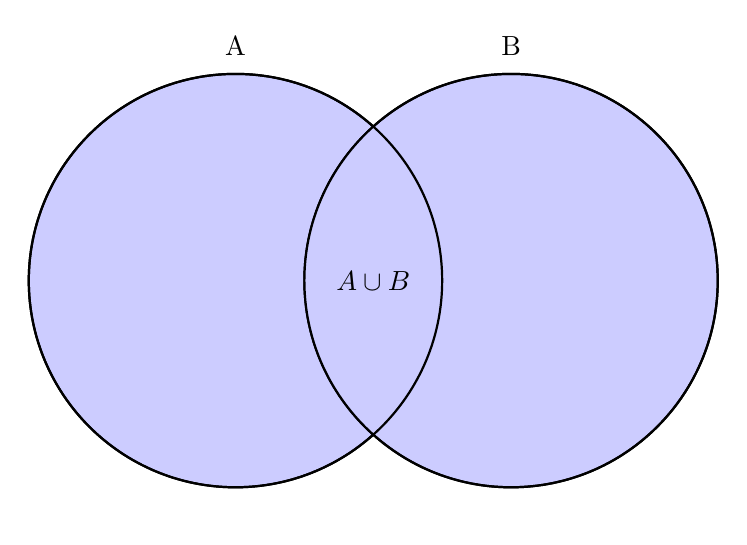
\begin{tikzpicture}[scale=1.75]
        \draw[thick, fill=blue!20] (2, 2) circle (1.5);
        \draw[thick, fill=blue!20] (4, 2) circle (1.5);
        
        \begin{scope}
            \clip (2, 2) circle (1.5);
            \fill[white] (4, 2) circle (1.5);
            \clip (2, 2) circle (1.5);
            \fill[blue!20] (4, 2) circle (1.5);
        \end{scope}

        \draw[thick] (2, 2) circle (1.5);
        \draw[thick] (4, 2) circle (1.5);
        
        \node at (2, 3.7) {A};
        \node at (4, 3.7) {B};
        
        \node at (3, 2) {\(A \cup B\)};
        
        \node at (3, 0.35) {};

        \node[overlay] at (0.2,3.75) {\(\bigcup\)};
    \end{tikzpicture}
}

\newpage
\subsubsection{Intersection $A \cap B$}
If $A$ and $B$ are sets, then their intersection is:
\figbox{$A \cap B = \left\{\forall x \in \bigcup \sht x \in A \land x \in B\right\}$}

\figbox{
    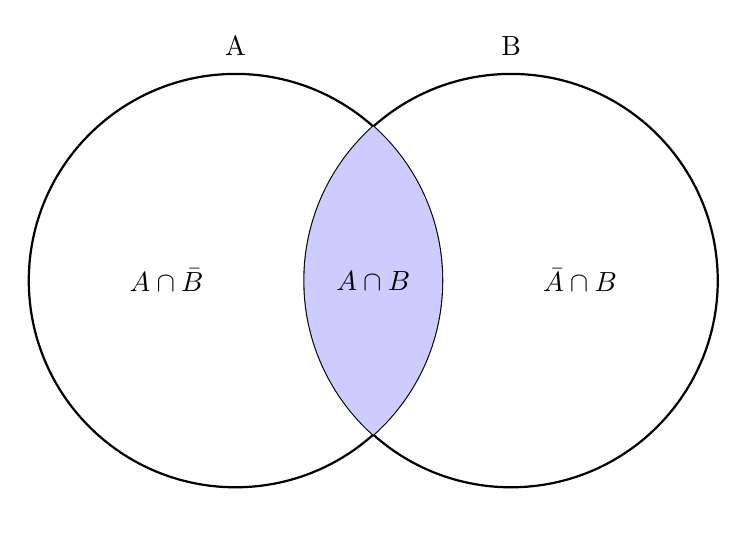
\begin{tikzpicture}[scale=1.75]
        
        \draw[thick] (2, 2) circle (1.5);
        \draw[thick] (4, 2) circle (1.5);
        \begin{scope}
            \clip (2, 2) circle (1.5);
            \fill[blue!20] (4, 2) circle (1.5);
        \end{scope}
        
        \node at (2, 3.7) {A};
        \node at (4, 3.7) {B};
        
        \node at (1.5, 2) {\(A \cap \bar{B}\)};
        \node at (4.5, 2) {\(\bar{A} \cap B\)};
        \node at (3, 2) {\(A \cap B\)};
        
        \node at (3, 0.35) {};

        \node[overlay] at (0.2,3.75) {\(\bigcup\)};
    \end{tikzpicture}
}

\subsubsection{Complement $\bar{A}$}
If $A$ is a set, its complement is:
\figbox{$\bar{A}=\left\{\forall x \in \bigcup \sht x \notin A\right\}$}

\begin{figure}[ht!]
    \begin{center}
            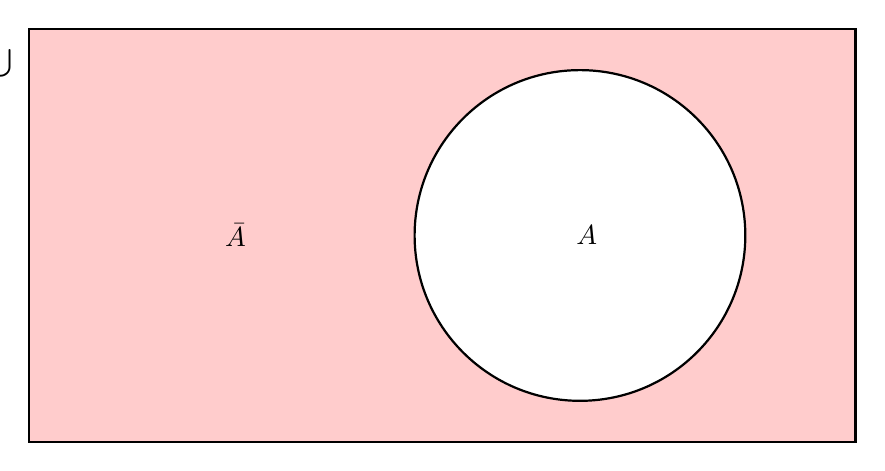
\begin{tikzpicture}[scale=1.75]
                
                \fill[red!20] (0, 0) rectangle (6, 3);
                \draw[thick] (0, 0) rectangle (6, 3);
        
                \fill[white] (4, 1.5) circle (1.2);
                \draw[thick] (4, 1.5) circle (1.2);
                
                \node at (1.5, 1.5) {\(\bar{A}\)};
                \node at (4.05, 1.5) {\(A\)};

                \node[overlay] at (-0.2,2.75) {\(\bigcup\)};
            \end{tikzpicture}
    \end{center}
\end{figure}

\newpage
\subsubsection{Difference between sets $\difference$}
If $A$ and $B$ are sets, then their difference is:
\figbox{$A \difference B = \left\{\forall x \in \bigcup \sht x \in A,\ x \notin B\right\}$}

\figbox{        
    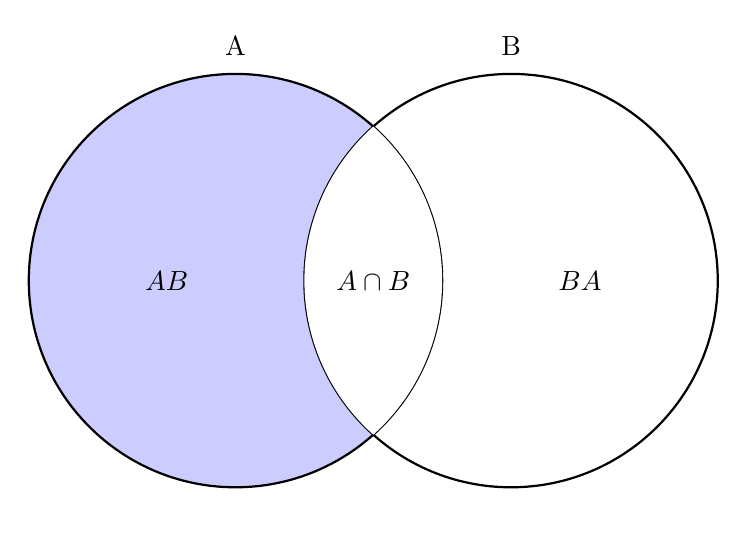
\begin{tikzpicture}[scale=1.75]
        \draw[thick, fill=blue!20] (2, 2) circle (1.5);
        \draw[thick] (4, 2) circle (1.5);
            
        \begin{scope}
            \clip (2, 2) circle (1.5);
            \fill[white] (4, 2) circle (1.5);
        \end{scope}
        
        \node at (2, 3.7) {A};
        \node at (4, 3.7) {B};
        
        \node at (1.5, 2) {\(A \difference B\)};
        \node at (4.5, 2) {\(B \difference A\)};
        \node at (3, 2) {\(A \cap B\)};
        
        \node at (3, 0.35) {};

        \node[overlay] at (0.2,3.75) {\(\bigcup\)};
    \end{tikzpicture}
}

\subsubsection{Symmetrical difference $\bigtriangleup$}
If $A$ and $B$ are sets, then their symmetrical difference is:
\figbox{$A \bigtriangleup B = (A \difference B) \cup (B \difference A)$}
\figbox{
    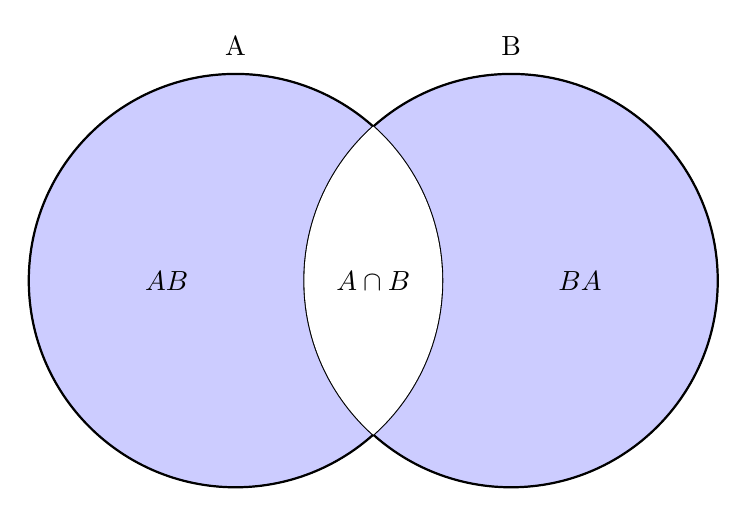
\begin{tikzpicture}[scale=1.75]
        \draw[fill=blue!20] (2, 2) circle (1.5);
        \draw[fill=blue!20] (4, 2) circle (1.5);
        
        \draw[thick] (2, 2) circle (1.5);
        \draw[thick] (4, 2) circle (1.5);
        
        \begin{scope}
            \clip (2, 2) circle (1.5);
            \fill[white] (4, 2) circle (1.5);
        \end{scope}
        
        \node at (2, 3.7) {A};
        \node at (4, 3.7) {B};
        
        \node at (1.5, 2) {\(A \difference B\)};
        \node at (4.5, 2) {\(B \difference A\)};
        \node at (3, 2) {\(A \cap B\)};
    \end{tikzpicture}
}

\newpage
\subsubsection{Disjoined sets (Empty sets) $\emptyset$}
$\emptyset :=$ the set containing zero elements:
\figbox{$A \cap B = \emptyset$}

\begin{figure}[ht!]
    \begin{center}
            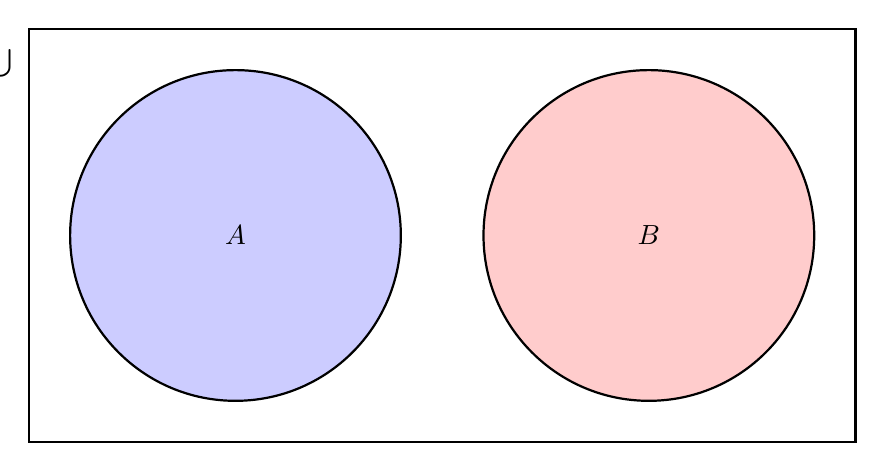
\begin{tikzpicture}[scale=1.75]
                
                \draw[thick] (0, 0) rectangle (6, 3);
        
                \fill[blue!20] (1.5, 1.5) circle (1.2);
                \draw[thick] (1.5, 1.5) circle (1.2);
                \fill[red!20] (4.5, 1.5) circle (1.2);
                \draw[thick] (4.5, 1.5) circle (1.2);
                
                \node at (1.5, 1.5) {\(A\)};
                \node at (4.5, 1.5) {\(B\)};
                            
                \node[overlay] at (-0.2,2.75) {\(\bigcup\)};
            \end{tikzpicture}
    \end{center}
\end{figure}

\newpage
\part{Algebra}
\section{Intervals in the real line}
Intervals describe what happens between two or more elements.

\subsection{Examples}
\subsubsection{Interval sets}
We have 4 cases:
\begin{itemize}
    \item $(a,b) = \left\{\forall x \in \mathbb{R} \sht a<x<b\right\}$;
    \item $\left[a,b\right) = \left\{\forall x \in \mathbb{R} \sht a\leq x<b\right\}$;
    \item $\left(a,b\right] = \left\{\forall x \in \mathbb{R} \sht a<x\leq b\right\}$;
    \item $\left[a,b\right] = \left\{\forall x \in \mathbb{R} \sht a\leq x\leq b\right\}$.
\end{itemize}

\nots{$a$ and $b$ are often called the ``end points'' of the interval;\\}

\subsubsection{Graphical examples}
$\forall x \in \mathbb{R},\ x \in \left[a,b\right]$
\begin{center}
    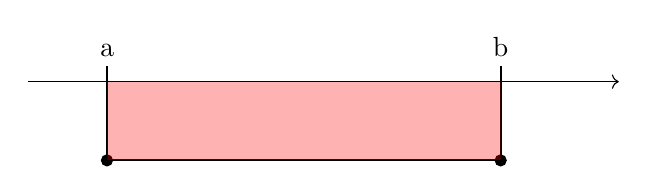
\begin{tikzpicture}
        %number line
        \draw[-] (-4,0) -- (3,0);
        \draw[thick] (-3,-0.2) -- (-3,0.2);
        \draw[thick] (2,-0.2) -- (2,0.2);
        
        %interval
        \draw[thick] (-3,-1) -- (2,-1);
        \draw[thick] (-3,0) -- (-3,-1);
        \draw[thick] (2,0) -- (2,-1);
        \filldraw[black] (-3,-1) circle (2pt);
        \filldraw[black] (2,-1) circle (2pt);
        
        %points
        \node[above] at (-3,0.2) {a};
        \node[above] at (2,0.2) {b};
        
        %arrow
        \draw[->] (3,0) -- (3.5,0);

        %area
        \filldraw [fill=red, draw=black, opacity=0.3] (-3,0) rectangle (2,-1);
    \end{tikzpicture}
\end{center}

\section{The extended line}
In the real line $\mathbb{R}$ we add $\pm \infty$.

\paragraph{Real line:} $(-\infty, +\infty) = \mathbb{R}$ 

\paragraph{Extended real line:} $\left[-\infty, +\infty\right] = \overline{\mathbb{R}}$

\vspace*{.5cm}
\begin{center}
    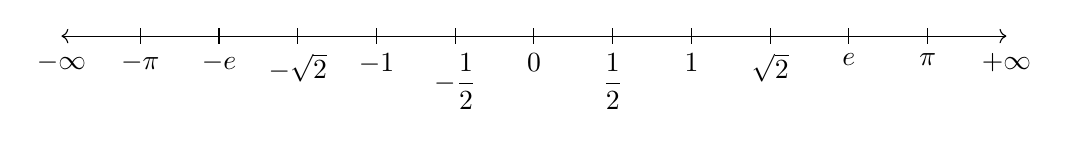
\begin{tikzpicture}
        \draw[->] (0,0) -- (6,0);
        \draw[<-] (-6,0) -- (0,0);

        \foreach \x/\label in {-5/{$-\pi$}, -4/{$-e$}, -3/{$-\sqrt{2}$}, -2/{$-1$}, -1/{$-\dfrac{1}{2}$}, 0/{$0$}, 1/{$\dfrac{1}{2}$}, 2/{$1$}, 3/{$\sqrt{2}$}, 4/{$e$}, 5/{$\pi$}} {
            \draw (\x,0.1) -- (\x,-0.1) node[below] {\label};
        }
        \node[below] at (-6,-0.1) {$-\infty$};
        \node[below] at (6,-0.1) {$+\infty$};
    \end{tikzpicture}
\end{center}

\rem{$\pm \infty \notin \mathbb{R}$}

\subsection{Properties}
\figbox{$\forall x \in \mathbb{R} \ \sht \ \infty > x \ \sht \ -\infty < 0$}

\subsection{Operation in the extended line}
If $a,b \in \mathbb{R}$, then $a+b,\; a-b,\; a\cdot b,\; \dfrac{a}{b} \text{ (with } b\neq 0 )$ stay the same

\subsubsection{Additions}
Let $\forall a \in \mathbb{R}$:
\begin{itemize}
    \item $a+\infty := \infty$;
    \item $a-\infty := -\infty$;
    \item $+\infty + \infty := +\infty$;
    \item $-\infty - \infty := -\infty$;
    \item $+\infty - \infty :=$ undefined.
\end{itemize}

\subsubsection{Moltiplications}
Let $\forall a \in \mathbb{R}$:
\begin{itemize}
    \item $+\infty \cdot +\infty := +\infty$;
    \item $-\infty \cdot +\infty := -\infty$;
    \item $-\infty \cdot (-\infty) := \infty$;
    \item $a \cdot \infty := \begin{cases}
        a > 0 &+\infty\\
        a < 0 &-\infty\\
        a = 0 & \text{undefined}
    \end{cases}$
    \item $a \cdot (-\infty):= \begin{cases}
        a > 0 &-\infty\\
        a < 0 &+\infty\\
        a = 0 &\text{undefined}
    \end{cases}$
    \item $\dfrac{a}{+\infty}=\dfrac{a}{-\infty} := 0$;
    \item $\dfrac{+\infty}{a}:= \begin{cases}
        a > 0 &+\infty\\
        a < 0 &-\infty\\
        a = 0 &+\infty
    \end{cases}$
    \item $\dfrac{-\infty}{a}:= \begin{cases}
        a > 0 &-\infty\\
        a < 0 &+\infty\\
        a = 0 &-\infty
    \end{cases}$
    \item $\dfrac{\infty}{\infty}:=$ undefined.
\end{itemize}

\section{Intervals including $\pm \infty$}
Intervals describe what happens between two or more elements, including $\pm \infty$.
\subsection{Examples}
\subsubsection{Interval sets}
Let $a \in \mathbb{R}$, then:
\begin{itemize}
    \item $(-\infty,a)=\left\{\forall x \in \mathbb{R} \sht x < a\right\}$;
    \item $(a, +\infty)=\left\{\forall x \in \mathbb{R} \sht x > a\right\}$;
    \item $(-\infty, a]=\left\{\forall x \in \mathbb{R} \sht x \leq a\right\}$;
    \item $[a,+\infty]=\left\{\forall x \in \mathbb{R} \sht x \geq a\right\}$;
    \item $(-\infty,+\infty)=\mathbb{R}$;
    \item $[-\infty,+\infty]=\overline{\mathbb{R}}$.
\end{itemize}

\subsubsection{Graphical examples}
$\forall x \in \mathbb{R},\ x \in\ \left[a,b\right]\ \cup\ \left] c, +\infty\right[$

\begin{center}
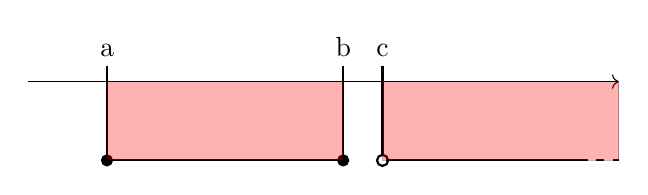
\begin{tikzpicture}
    %number line
    \draw[-] (-3,0) -- (4,0);
    \draw[thick] (-2,-1) -- (-2,0.2);
    \draw[thick] (1,-1) -- (1,0.2);
    \draw[thick] (1.5,-0.95) -- (1.5,0.2);
    
    %intervals
    \draw[thick] (-2,-1) -- (1,-1);
    \filldraw[black] (-2,-1) circle (2pt);
    \filldraw[black] (1,-1) circle (2pt);
    \draw[thick] (1.55,-1) -- (4,-1);
    \draw[thick, dashed] (4,-1) -- (4.5,-1);
    \draw[thick] (1.5,-1) circle (2pt);
    
    %points
    \node[above] at (-2,0.2) {a};
    \node[above] at (1,0.2) {b};
    \node[above] at (1.5,0.2) {c};
    
    %arrow
    \draw[->] (4,0) -- (4.5,0);

    %area
    \filldraw [fill=red, draw=black, opacity=0.3] (-2,0) rectangle (1,-1);
    \filldraw [fill=red, draw=black, opacity=0.3] (1.5,0) rectangle (4.5,-1);
\end{tikzpicture}
\end{center}
\vspace*{.5cm}
\nots{The union of two or more intervals where $x \in \mathbb{R}$
is denoted by the symbol $\cup$.}

\section{The absolute value function}
The absolute value is an operator that returns the positive value of a
number, regardless of its original sign.

Let $x \in \mathbb{R}$, then:
\figbox{$|x|=\begin{cases}
    x \text{ if} &x \geq 0\\
    x \text{ if} &-x < 0
\end{cases}$}

\subsection{Graph of absolute value functions}
Let's plot the function $y=|x|$:
\begin{figure}[ht!]
    \centering
    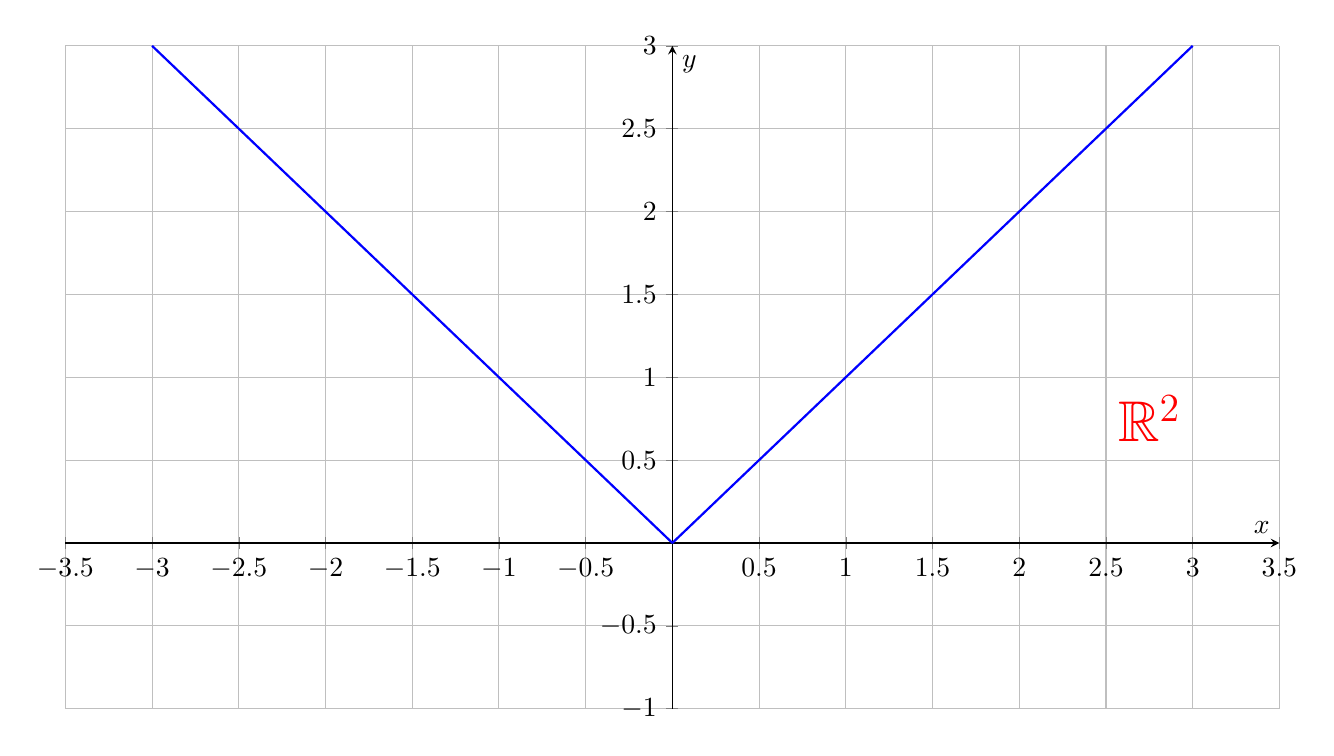
\begin{tikzpicture}
        \begin{axis}[
            axis lines = middle,
            xlabel = {$x$},
            ylabel = {$y$},
            domain=-3:3,
            samples=1500,
            xmin=-3.5, xmax=3.5,
            ymin=-1, ymax=3,
            grid=major,
            width=17cm, height=10cm
        ]
            \addplot[blue, thick] {abs(x)};
            \node[red] at (2.75,.75) {\huge $\mathbb{R}^2$};
            \end{axis}
    \end{tikzpicture}
\end{figure}

\subsection{Properties}
Let $a,b \in \mathbb{R}$, then:
\begin{itemize}
    \item $|a\cdot b|=|a| \cdot |b|$;
    \item $\left\vert\dfrac{a}{b}\right\vert= \dfrac{|a|}{|b|} $ for $b \neq 0$;
    \item $|a\pm b| \neq |a|\pm |b|$.
\end{itemize}

\newpage
\subsection{Triangular inequalities}
Let $a,b \in \mathbb{R}$, then:
\figbox{\begin{minipage}{0.135\textwidth}
    \begin{center}
        $|a|+|b| \geq |a+b|$\\
        $|a|-|b| \leq |a-b|$ 
    \end{center}
\end{minipage}
}

\section{Concept of functions}
Let's take any two sets $A\left\{a,b,c,d,e,f,g\right\}$ and $B\left\{a_1,b_1,c_1,d_1,e_1,f_1,g_1\right\}$.

\figbox{ \hspace*{-1cm}
    \begin{minipage}{0.12\textwidth}
        \vspace*{-0.4cm}
        \begin{align*}
            f: A &\implies B \\
            a &\longmapsto f(a)
        \end{align*}
    \end{minipage}
}

A function is a relation between the sets $A$ and $B$, according to which we
associate to each element of $A$ one and only one element of $B$:

\figbox{
    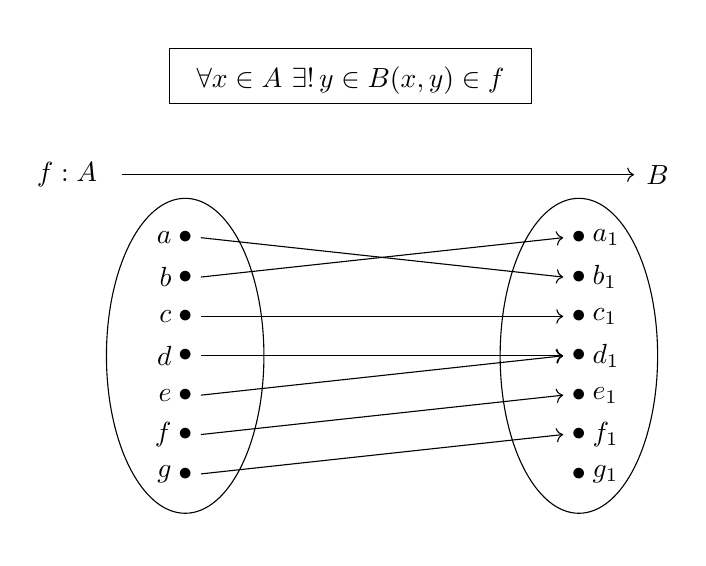
\begin{tikzpicture}

        %formula
        \node at (2.1,3.5) {$\forall x \in A\ \exists!\, y \in B \sht (x,y) \in f$};
        \draw (-0.2,3.2) rectangle (4.4,3.9);

        %sets A and B
        \draw (0,0) ellipse (1 and 2);
        \draw (5,0) ellipse (1 and 2);
        \node at (-1.5,2.3) {$f:A$};
        \node at (6,2.3) {$B$};
        \draw[->] (-0.8,2.3) -- (5.7,2.3);
        
        %set A
        \node at (0,-1.5) {$\bullet$};
        \node[left] at (-0.05,-1.5) {$g$};
        \node at (0,-1) {$\bullet$};
        \node[left] at (-0.05,-1) {$f$};
        \node at (0,-0.5) {$\bullet$};
        \node[left] at (-0.05,-0.5) {$e$};
        \node at (0,0) {$\bullet$};
        \node[left] at (-0.05,0) {$d$};
        \node at (0,0.5) {$\bullet$};
        \node[left] at (-0.05,0.5) {$c$};
        \node at (0,1) {$\bullet$};
        \node[left] at (-0.05,1) {$b$};
        \node at (0,1.5) {$\bullet$};
        \node[left] at (-0.05,1.5) {$a$};
        
        %set B
        \node at (5,-1.5) {$\bullet$};
        \node[right] at (5.05,-1.5) {$g_1$};
        \node at (5,-1) {$\bullet$};
        \node[right] at (5.05,-1) {$f_1$};
        \node at (5,-0.5) {$\bullet$};
        \node[right] at (5.05,-0.5) {$e_1$};
        \node at (5,0) {$\bullet$};
        \node[right] at (5.05,0) {$d_1$};
        \node at (5,0.5) {$\bullet$};
        \node[right] at (5.05,0.5) {$c_1$};
        \node at (5,1) {$\bullet$};
        \node[right] at (5.05,1) {$b_1$};
        \node at (5,1.5) {$\bullet$};
        \node[right] at (5.05,1.5) {$a_1$};
        
        %arrows
        \draw[->] (0.2,-1.5) -- (4.8,-1);
        \draw[->] (0.2,-1) -- (4.8,-0.5);
        \draw[->] (0.2,-0.5) -- (4.8,0);
        \draw[->] (0.2,0) -- (4.8,0);
        \draw[->] (0.2,0.5) -- (4.8,0.5);
        \draw[->] (0.2,1) -- (4.8,1.5);
        \draw[->] (0.2,1.5) -- (4.8,1);

        %spacer
        \node at (0,4.05) {\phantom{}};
        \node at (0,2.6) {\phantom{}};
        \node at (0,-2.2) {\phantom{}};
    \end{tikzpicture}
}

\nots{$f(a)=b_1,\ f(b)=a_1,\ f(c)=c_1,\ f(d)=d_1,$ ...}

Each point in set $A$ is associated with one element of $B$. However, it is
possible for more than two elements of $A$ to point to the same element of $B$.

\figbox{The set $A$ is called \textit{domain} of $f$. The set $B$ is called the \textit{codomain} of $f$.}

\subsection{Image (Range)}
Let $f: X \implies Y$ be a function. The image of $f$ is defined as:
\figbox{\text{Im($f$)}$=\{y \in Y \sht y=f(x),\ x \in X\}$}

Easily, the image is the set containing all the elements of the set $B$ associated
with the elements of the set $A$.

\newpage
\section{Linear function}
\subsection{Cartesian diagram}
\begin{center}
    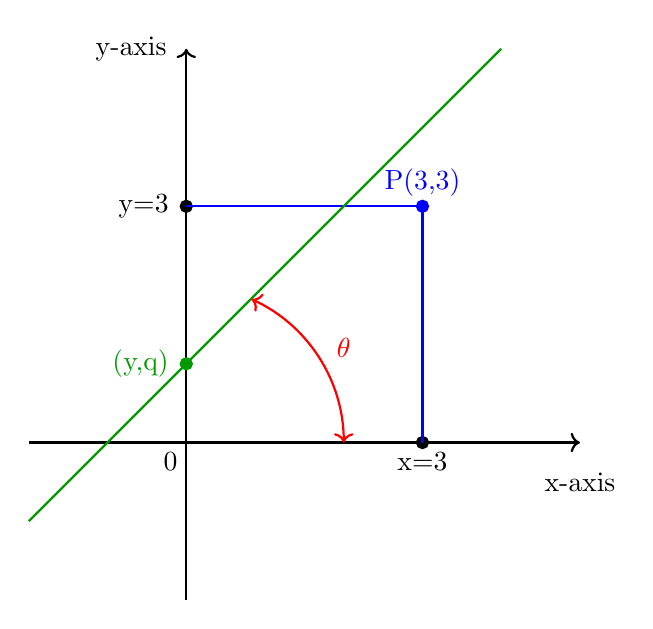
\begin{tikzpicture}
        \definecolor{darkgreen}{rgb}{0.0, 0.6, 0.0}

        \draw[thick][->] (-2,0) -- (5,0);
        \draw[thick][->] (0,-2) -- (0,5);
        \node at (5,-.5) {x-axis};
        \node at (-.7,5) {y-axis};
        \draw[fill, thick] (3,0) circle (2pt);
        \node[below] at (3,0) {x=3};
        \draw[fill, thick] (0,3) circle (2pt);
        \node[left] at (-.1,3) {y=3};
        \draw[blue, thick] (3,0) -- (3,3);
        \draw[blue,thick] (0,3) -- (3,3);
        \draw[fill, blue, thick] (3,3) circle (2pt);
        \node[blue, above] at (3,3) {P(3,3)};
        \node[below] at (-0.2,0) {0};
        
        \draw[darkgreen, thick] (-2,-1) -- (4,5);
        \draw[fill, darkgreen, thick] (0,1) circle (2pt);
        \node[darkgreen, left] at (-0.1,1) {(y,q)};

        \draw[red, thick, <->] (2,0) arc[start angle=0,end angle=65.5,radius=2];
        \node[red] at (2,1.2) {$\theta$};

    \end{tikzpicture}
\end{center}

\subsection{Straight line}
Let A and B be any two distinct points, then there is one and only one
line passing through A and B.

\subsection{Slope-intercept equation}
Let $m,q \in \mathbb{R}$, then
\figbox{$y=mx+q$}

\begin{itemize}
    \item $m$: slope;
    \item $q$: vertical intercept.
\end{itemize}

\subsubsection{Slope}
The slope of a line can be calculated with the equation
\figbox{$m=\dfrac{y_B-y_A}{x_B-x_A}=\dfrac{\Delta y}{\Delta x} = \tan{(\theta)}$}

We have three different slope outcomes:
\begin{itemize}
    \item $m>0$, the line is increasing;
    \item $m=0$, the line is stable;
    \item $m<0$, the line is decreasing. 
\end{itemize}

\wrn{This works only if $x_B \neq x_A$.}

\subsubsection{Drawing}
\begin{center}
    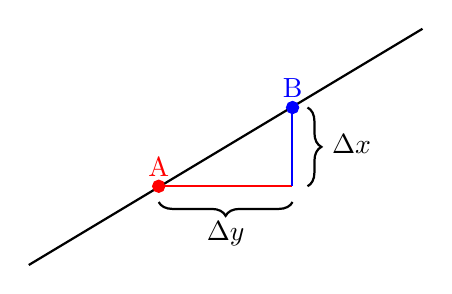
\begin{tikzpicture}
        \draw[thick] (0,0) -- (5,3);
        \draw[fill, thick, red] (1.65,1) circle (2pt);
        \node[above, red] at (1.65,1) {A};
        \draw[fill, thick, blue] (3.35,2) circle (2pt);
        \node [above, blue] at (3.35, 2) {B};

        %slope
        \draw[thick, red] (1.65,1) -- (3.34,1);
        \draw[thick, blue] (3.34,2) -- (3.34,1);

        %braces
        \draw[decorate,decoration={brace,amplitude=5pt},thick] (3.54,2) -- (3.54,1);
        \node at (4.1,1.53) {$\Delta x$};
        \draw[decorate,decoration={brace,amplitude=5pt},thick] (3.35,0.8) -- (1.65,0.8);
        \node at (2.5,0.4) {$\Delta y$};
    \end{tikzpicture}
\end{center}

\subsection{Vertical lines}
The more the value of m increases, the closer the line will get to the vertical,
without ever reaching it.

Let $c \in \mathbb{R}$, then $x=c$.

Vertical lines cannot be written as a function.

\section{Equation of a line}
Let $m,x_A,y_A \in \mathbb{R}$ and $A(x_A, y_A)$, then
\figbox{$y-y_A=m(x-x_A)$}

e.g.: Find the line with $m=-1$ and $A(1,0)$.
\[
    y-0=-1(x-1) \implies y=-x+1
\]
\hspace{.75cm} Points: $A(1,0);\ B(0,1)$


\begin{center}
    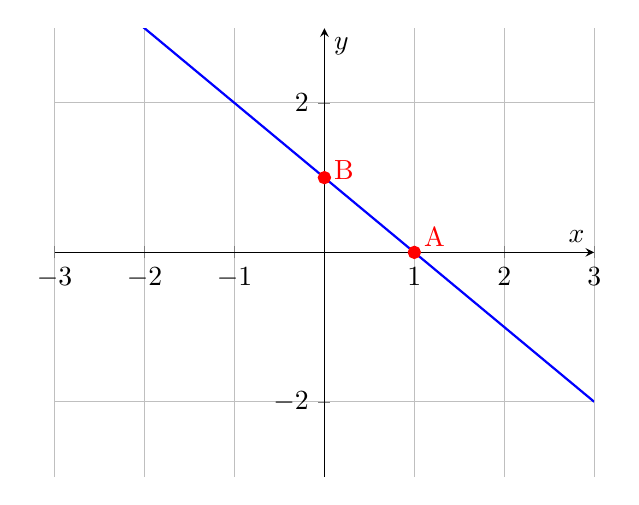
\begin{tikzpicture}
        \begin{axis}[
                axis lines = middle,
                xlabel = $x$,
                ylabel = $y$,
                grid = both,
                xmin=-3, xmax=3,
                ymin=-3, ymax=3,
                domain=-3:3
            ]
            \addplot[color=blue, thick] {-x + 1};
            \draw[fill, red, thick] (1,0) circle (2pt);
            \node[right,red] at (1,.2) {A};
            \draw[fill,red,thick] (0,1) circle (2pt);
            \node[right,red] at (0,1.1) {B};
        \end{axis}
    \end{tikzpicture}
\end{center}

\subsection{General equation in a cartesian diagram}
\figbox{$ax+by+c=0$}

\rem{\begin{itemize}
    \item All the lines can be described with this kind of equation;
    \item When $b=0$, $a \neq 0$, then $ax=-c \implies x=\dfrac{-c}{a} \in \mathbb{R}$;
    \item When $b \neq 0$, then $y=-\dfrac{a}{b}x -\dfrac{c}{b}$,
        where $m=-\dfrac{a}{b}$ and $q=-\dfrac{c}{b}$.
\end{itemize}}

\newpage
\section{Increasing and decreasing functions}
Let $f:[a,b] \longrightarrow \mathbb{R}$

\nots{if your replace $[a,b]$ with $\mathbb{R}$, you obtain the definition in the whote $\mathbb{R}$.}

\subsection{Increasing functions}
\begin{itemize}
    \item $f$ is increasing if $\forall x_1,x_2 \in [a,b] \sht x_2>x_1$, then $f(x_2)\geq f(x_1)$;
    \item $f$ is strictly increasing if $\forall x_1,x_2 \in [a,b] \sht x_2>x_1$, then $f(x_2)>f(x_1)$.
\end{itemize}

\subsection{Decreasing functions}
\begin{itemize}
    \item $f$ is decreasing if $\forall x_1,x_2 \in [a,b] \sht x_2>x_1$, then $f(x_2)\leq f(x_1)$;
    \item $f$ is strictly decreasing if $\forall x_1,x_2 \in [a,b] \sht x_2>x_1$, then $f(x_2)<f(x_1)$.
\end{itemize}

\section{Inverse function}
Let's take any two sets $A$ and $B$.

A function $f: A \implies B$ is invertible if there exists another
function $f^{-1}: B \implies A$, called the inverse function, such that:

\figbox{\begin{minipage}{3.6cm}
    $\forall x \in A,\ f^{-1}(f(x)) = x$ \vspace*{-.25cm}\\
    $\forall y \in B,\ f(f^{-1}(y)) = y$
\end{minipage}}

\wrn{A function is invertible if and only if it is bijective.}

\subsection{Facts about inverse functions}
\pph{1)}
Let $f:D\implies \mathbb{R}$

$f$ is invertible in $D$ when:
\begin{itemize}
    \item $f$ is strictly increasing;
    \item $f$ is strictly decreasing.
\end{itemize}

\pph{2)}
Let $f:D \implies \mathbb{R}$

$f$ is invertible when $f^{-1}:$ Im$(f) \implies D$.

\newpage
\section{Expressions and factorization}
\subsection{Expressions, terms and factors}
\subsubsection{Expressions}
An expression is any formula containing numbers, variables, operations, and
brackets.
\figbox{$y=ax^2+bx\cdot c$}

\subsection{Terms}
A term is any part of the expression separated by ``$+$'' or ``$-$''.
\figbox{$y = \underbrace{ax^2}_{term} + \underbrace{bx \cdot c}_{term}$}

\subsubsection{Factors}
Each term can be split into a product of factors.
\figbox{$x \cdot y \cdot (a-b) \cdot 24 = x \cdot y \cdot (a-b) \cdot 2 \cdot 2 \cdot 2 \cdot 3$}

\underline{Notice}: the process of splitting a term into several factors is called ``factorization''.\\
\phantom{} \hspace{1cm} The goal of a factorization is to factorize an expression as much as possible.

\subsubsection{Common factor}
Any expression made of terms is composed of several factors.
\figbox{$x^2+x^3+x= x(x+x^2+1),\ \forall x \in \mathbb{R}$}

\subsection{Notable producs}
\begin{itemize}
    \item $(a+b)^2=a^2+2ab+b^2$ (square of a binomial);
    \item $(a-b)^2=a^2-2ab+b^2$ (square of a binomial);
    \item $(a-b)(a+b)=a^2-b^2$ (difference of squares);
    \item $(a+b)(a^2-ab+b^2)=a^3+b^3$ (sum of cubes);
    \item $(a-b)(a^2+ab+b^2)=a^3-b^3$ (difference of cubes).
\end{itemize}

\underline{Remark}: notable products are useful to factorize expressions when we don't know a common factor.

\newpage
\section{Polynomial function}
Let $n \in \mathbb{N^*}$, then a polynomial is the sum or difference of n-monomials. 

\section{Classification of polynomials}
Polynomials can be classified using two criteria: 
\begin{enumerate}
    \item the number of \textbf{terms};
    \item the \textbf{degree} of the polynomial.
\end{enumerate}
\begin{center}
    $\begin{aligned}
        &\begin{array}{|c|c|l|c|}
        \hline \rule{0pt}{13pt} \text { Number of Terms } & \text { Name } & \text { Example } & \text { Degree } \\
        \hline \rule{0pt}{13pt} \text { One } & \text { Monomial } & ax^2 & \text { 1 } \\
        \hline \rule{0pt}{13pt} \text { Two } & \text { Binomial } & ax^2-b x & \text { 2 } \\
        \hline \rule{0pt}{13pt} \text { Three } & \text { Trinomial } & ax^2-b x+c & \text { 3 } \\
        \hline \rule{0pt}{13pt} \text { Four or more } & \text { Polynomial } & a_n x^n-a_1 x^{n-1}+a_2x^{n-2}\cdots a_0& \text { n-degree } \\
        \hline
        \end{array}
    \end{aligned}$
\end{center}
\vspace*{.3cm}
\rem{The degree of a polynomial is the largest exponent of its monomials.}

\section{Symmetrical functions}
Let $y = kx^n$, then we plot:
\subsection{$n$ odd}
\figbox{$f(-x)=-f(x), \quad \forall x \in \mathbb{R}$}

\subsubsection{Graph examples}
\begin{figure*}[htbp!]
    \centering
    \begin{subfigure}{0.45\textwidth}
        \centering
        \begin{tikzpicture}[scale=.95]
            \begin{axis}[
                domain=-2:2,
                samples=100,
                axis lines=middle,
                xlabel=$x$, ylabel={$y$},
            ]
            \addplot[color=blue, thick]{(x/2)^3};
            \end{axis}
        \end{tikzpicture}
        \caption*{$k > 0$}
    \end{subfigure}
    \hfill
    \begin{subfigure}{0.45\textwidth}
        \centering
        \begin{tikzpicture}[scale=.95]
            \begin{axis}[
                domain=-2:2,
                samples=100,
                axis lines=middle,
                xlabel=$x$, ylabel={$y$},
            ]
            \addplot[color=red, thick]{-(x/2)^3};
            \end{axis}
        \end{tikzpicture}
        \caption*{$k < 0$}
    \end{subfigure}
\end{figure*}

\newpage
\subsection{$n$ even}
\figbox{$f(-x)=f(x), \quad \forall x \in \mathbb{R}$}

\subsubsection{Graph examples}
\begin{figure}[htbp]
    \centering
    \begin{subfigure}{0.45\textwidth}
        \centering
        \begin{tikzpicture}[scale=.95]
            \begin{axis}[
                domain=-2:2,
                samples=100,
                axis lines=middle,
                xlabel=$x$, ylabel={$y$},
            ]
            \addplot[color=blue, thick]{(x/2)^2};
            \end{axis}
        \end{tikzpicture}
        \caption*{$k > 0$ \\ Concave up}
    \end{subfigure}
    \hfill
    \begin{subfigure}{0.45\textwidth}
        \centering
        \begin{tikzpicture}[scale=.95]
            \begin{axis}[
                domain=-2:2,
                samples=100,
                axis lines=middle,
                xlabel=$x$, ylabel={$y$},
            ]
            \addplot[color=red, thick]{-(x/2)^2};
            \end{axis}
        \end{tikzpicture}
        \caption*{$k < 0$\\Concave down}
    \end{subfigure}
\end{figure}

\defs{\begin{itemize}
    \item a function $y=f(x)$ is called \textbf{odd} if it is symmetric with
    respect to the origin;
    \item a function $y=f(x)$ is called \textbf{even} if it is symmetric
    with respect to the y-axis.
\end{itemize}}

\subsection{General case}
Let $y=p(x)$, where $p(x)$ is any polynomial with real coefficients:
\figbox{$p(x)=a_n \cdot x^n + a_{n-1} \cdot x^{n-1} + a_{n-2} \cdot x^{n-2} + ... + a_{2} \cdot x^{2} + a_{1} \cdot x^{1} + a_{0}$}

where:
\begin{itemize}
    \item $n \in \mathbb{N}$;
    \item $n=\deg(p(x))$;
    \item $a_n=$ leading coefficient.
\end{itemize}

\figbox{\large $\displaystyle p(x)=\sum^{n}_{i=0} a_i \cdot x^i$}

\subsection{Symmetry of a polynomial}
Let $y=p(x)$ be a polynomial function, then:
\pph{1)}
$y=p(x)$ is odd iff all the degrees of all the terms of
$p(x)$ are odd;

\pph{2)}
$y=p(x)$ is even iff all the degrees of all the terms of
$p(x)$ are even;

\pph{3)}
$y=p(x)$ has mixed degrees, $p(x)$ is neither odd nor even.

\newpage
\section{Intersection with axis}
\subsection{Vertical intersection}
Let $y=f(x)$ be any function, then we solve for $y$:
\figbox{$\begin{cases}
    x = 0 \\
    y=f(0)
\end{cases}$}

\subsection{Zeros of a function}
Let $y=f(x)$ be any function, then we solve for $x$:
\figbox{$\begin{cases}
    y = 0 \\
    0 = f(x)
\end{cases}$}

\subsection{Graph example}
\begin{center}
    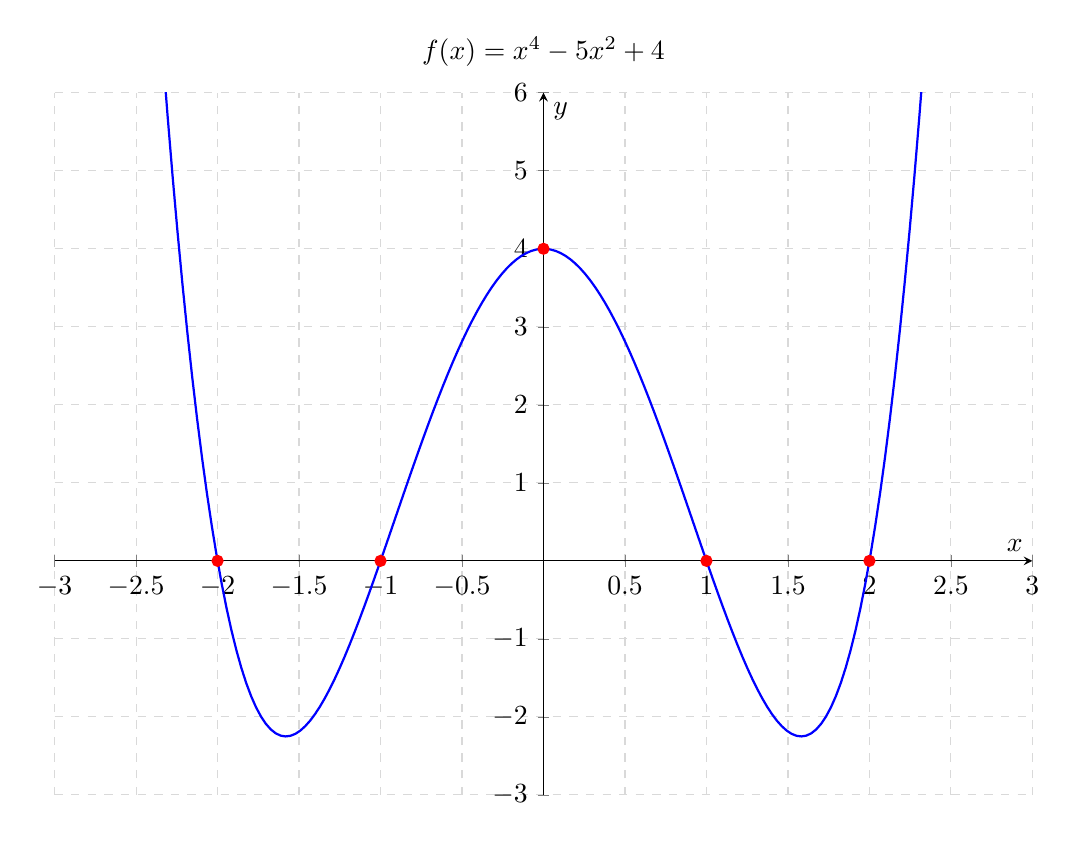
\begin{tikzpicture}
        \begin{axis}[
          title = {$f(x)=x^4-5x^2+4$},
          axis lines = middle,
          xlabel = $x$,
          ylabel = $y$,
          xmin = -3, xmax = 3,
          ymin = -3, ymax = 6,
          samples = 200,
          domain = -3:3,
          clip = true,
          grid = both,
          grid style = {dashed, gray!30},
          width = 14cm,
          height = 10.5cm,
        ]
        \addplot [blue, thick] {x^4 - 5*x^2 + 4};
        
        \addplot [
          only marks,
          mark=*,
          mark options={color=red},
        ] coordinates {
          (-2, 0) (-1, 0) (1, 0) (2, 0)
        };
        
        \addplot [
          only marks,
          mark=*,
          mark options={color=red},
        ] coordinates {
          (0, 4)
        };
        \end{axis}
    \end{tikzpicture}      
\end{center} 

\newpage
\section{Dominant elements in a function approaching $\pm \infty$}
As $x$ approaches $\pm \infty$, the term with the highest degree in a
polynomial function dominates the behavior of the function.
\figbox{$p(x)$ has, as a dominant, the element $a_n$ with the highest degree $x^n$}

\subsection{Order of dominance}
\subsubsection{Approaching to +$\infty$}
Let $n \in \mathbb{N},\ m \in \mathbb{N},\ 2<n<m$, then:

\figbox{$\ln(x) < x < x^n < x^m < n^x < m^x < x^x$}

In these cases, we always have $x \implies +\infty \implies p(x)\implies +\infty$

\subsubsection{Approaching to -$\infty$}
Let $\lambda > 2$ and odd,\ $k > 2$ and even.

\figbox{
  \begin{minipage}{3.25cm}
    $x^\lambda < -x^2 < x^1 < 0$ \\
    $-x^k < -x^2 < x^1 < 0$
  \end{minipage}
}

Functions like $x^\lambda$ (with $\lambda$ odd) and $-x^k$ (with $k$ even)
both approach $-\infty$, but at different rates.

\subsubsection{Dominance in rational functions}
When the dominant element is at the numerator:
\figbox{$\dm \lim_{x \to \infty} \dfrac{x^n}{x^{n-1}} = \infty$}

When the dominant element is at the denominator:
\figbox{$\dm \lim_{x \to \infty} \dfrac{x^{n-1}}{x^n} = 0$}

When we have the same degree either in the numerator and in the denominator:
\figbox{$\dm \lim_{x \to \infty} \dfrac{ax^n}{bx^n} = \dfrac{a}{b}$}

\defs{\textbf{horizontal asymptote} appears when $x$ approaches to $\infty$,
which implies that $y$ approaches to a number $A$ different from $\pm \infty$}

\newpage
\section{Exponential and logarithm functions}
The relationship between exponentials and logarithms is based on the following formula:
\figbox{$\dm a^{\log_a(x)} = x \Longleftrightarrow \log_a(a^x) = x$}

\subsection{Exponentials}
\subsubsection{General equation}
Let $\alpha \in \mathbb{R}^*_+$,\ $x \in \mathbb{R}$, and $a>1$, then:

\figbox{$y=\alpha \cdot a^x$}

\subsubsection{Euler's number}
Euler's number is defined by the limit:
\figbox{$\dm e = \lim_{n \to \infty} {\left(1+\dfrac{1}{n}\right)}^n \approx 2.718\cdots$}

Alternatively, it can be expressed as:
\figbox{$\dm e = \sum_{n=0}^\infty \frac{1}{n!} $}

\subsection{Logarithms}
\subsubsection{Natural logarithm}
The inverse function of the Euler's exponential function:
\figbox{$\dm f(x)=e^x \Longleftrightarrow h(x)=\ln(x)$}

\rem{the domain of $\ln(x)$ is D$_n:\ \forall x \in \mathbb{R}^{*}_{+}$}

\subsubsection{Logarithms with arbitrary bases}
The inverse function of any arbitrary exponential function:
\figbox{$\dm f(x)=n^x \Longleftrightarrow h(x)=\log_{n}(x)$}

Alternatively, it can be expressed as:
\figbox{$\dm \log_a (x) = \frac{\ln(x)}{\ln(a)}$}

\subsubsection{Common logarithm}
The common logarithm uses base 10:
\figbox{$\dm \log_{10}(x)=\frac{\ln(x)}{\ln(10)}$}

\newpage
\subsection{Exponential growth}
\figbox{$N(t)=N_0\cdot e^{kt}$}

\section{Composite functions}
Let $y=f(x)$ and $z=g(y)$ be two functions, then:

\figbox{$z=g(f(x))$}

\subsection{Examples}
\pph{1)}
Let $f(x)=x^2+4x$ and $g(y)=y^2+\cos(y)$ be two functions, then:

\[g(f(x))=\left(x^2+4x\right)^2+\cos(x^2+4x)\]

\pph{2)}
Let $f(x)=x^3,\ h(x)=\arctan(x)$ and $g(x)=\ln(x)$ be functions, then:

\[
  g(h(f(x)))=\ln(\arctan(x^3))
\]

\newpage
\part{Trigonometry}
\section{Trigonometry}
\subsection{Conversion table of degrees and radians}
\begin{center}
    \begin{tabular}{|c|c|c|c|c|c|c|c|c|}
        \hline
        \textbf{Angles (in Degrees)} & \rule{0pt}{15pt} $0^\circ$ & $30^\circ$ & $45^\circ$ & $60^\circ$ & $90^\circ$ & $180^\circ$ & $270^\circ$ & $360^\circ$ \\
        \hline
        \textbf{Angles (in Radians)} & \rule{0pt}{15pt} $0^{\rad}$ & $\pi/6^{\rad}$ & $\pi/4^{\rad}$ & $\pi/3^{\rad}$ & $\pi/2^{\rad}$ & $\pi^{\rad}$ & $3\pi/2^{\rad}$ & $2\pi^{\rad}$ \\
        \hline
        $\sin(\theta)$ & \rule{0pt}{15pt} 0 & $1/2$ & $\sqrt{2}/2$ & $\sqrt{3}/2$ & 1 & 0 & $-1$ & 0 \\
        \hline
        $\cos(\theta)$ & \rule{0pt}{15pt} 1 & $\sqrt{3}/2$ & $\sqrt{2}/2$ & $1/2$ & 0 & $-1$ & 0 & 1 \\
        \hline
        $\tan(\theta)$ & \rule{0pt}{15pt} 0 & $\sqrt{3}/3$ & 1 & $\sqrt{3}$ & $\infty$ & 0 & $\infty$ & 0 \\
        \hline
    \end{tabular}
\end{center}
\phantom{}

\underline{Remark}:

\begin{center}
    $\dm \cos(2\pi+\theta) = \cos(\theta) \qquad | \qquad
    \sin(2\pi+\theta) = \sin(\theta)$
\end{center}

\underline{Remark}:
Let $\forall k \in \mathbb{Z},\ \forall \theta \in \mathbb{R}$, then:
\figbox{$\cos(\theta + 2\pi k)=\cos(\theta)$}

\subsection{Trigonometric functions in the unit circle}
\begin{center}
    \begin{tikzpicture}[scale=3.75]
        \definecolor{darkgreen}{rgb}{0.0, 0.7, 0.0}
        %axes
        \draw[thick, ->] (-1.5,0) -- (1.5,0) node[right] {$x$};
        \draw[thick, ->] (0,-1.5) -- (0,1.5) node[above] {$y$};
        \node at (-0.06, -0.06) {$O$};
        \draw (0,0) circle (1);
    
        %theta angle
        \draw[thick, blue] (0,0) -- (0.866,0.5) node[right] {$P(x,y)$};
        \draw[dashed, blue] (0,0) -- (0.866,-0.5) node[right] {\ $P'(x,y')$};
        \draw[<->] (0.3,0) arc (0:30:0.3);
        \node at (0.35,0.10) {$\theta$};

        %dash
        \draw[dashed] (0.866,0.5) -- (0,0.5);
        \draw[dashed] (0.866,0) -- (0.866,-0.5);

        %projections
        \draw[thick, red] (0,0) -- (0.866, 0) node[midway, below] {$\cos \theta$};
        \draw[thick, darkgreen] (0.866,0) -- (0.866, 0.5) node[midway, left] {$\sin \theta$};
    
        %labels
        \node at (1.075, 0.05) {1};
        \node at (-0.05, 1.1) {1};
        \node at (-1.075, 0.05) {-1};
        \node at (-0.05, -1.1) {-1};
        \node at (1, 1) {I};
        \node at (-1, 1) {II};
        \node at (-1, -1) {III};
        \node at (1, -1) {IV};

        %others
        \draw (0.866,0) rectangle (0.816,0.05);
        \node[below] at (0.93,0) {$H$};
    \end{tikzpicture}
\end{center}
\vspace*{.5cm}
\rem{the circle has center in the origin $O$, radius $= 1$ and function $x^2+y^2=1$}

Trigonometric functions can be extended to angles beyond 0 and 90$^\circ$
using the unit circle. For an angle $\theta$ in the unit circle:
\figbox{$\dm \sin \theta := y\ \ |\ \cos \theta := x\ \ |\ \tan \theta := \frac{y}{x}$}

\subsubsection{Property 1 -- Domain and range}
Because we are inside a circle of radius 1:
\begin{itemize}
    \item $-1 \leq \cos(\theta) \leq 1$;
    \item $-1 \leq \sin(\theta) \leq 1$.
\end{itemize}

\subsubsection{Property 2 -- Trigonometric identity}
Because we have a 90$^\circ$ angle, we can use Pythagoras: 
\figbox{$\vv{OH}^{\,2}+\vv{PH}^{\,2}=\vv{OP}^{\,2}$}

Let $\dm \forall \theta \in \mathbb{R}$, then we can compute the following trigonometric identity:
\figbox{$\dm \sin^2(\theta) + \cos^2(\theta) = 1$}

\subsection{Tangent}
A tangent of an angle is exactly the slope of a line:
\figbox{$\dm m = \frac{\Delta y}{\Delta x} = \tan(\theta)=\frac{\sin(\theta)}{\cos(\theta)}$}

\underline{Remark}: the tangent is not defined when the angle is $\dfrac{\pi}{2}$
or $\dfrac{3\pi}{2}$, that is when we have a vertical line.

\subsection{Domain of trigonometric functions}
\figbox{
    \begin{minipage}{6.5cm}
        \hspace*{-.2cm}
        $\begin{array}{rcl} \vspace*{.15cm}
            y\ =&\!\! \cos(x), \quad &x\rad \in \mathbb{R}\\ \vspace*{.15cm}

            y\ =&\!\! \sin(x), \quad &x\rad \in \mathbb{R}\\ 

            y\ =&\!\! \tan(x), \quad &x\rad \in \mathbb{R} \difference \left\{\dfrac{\pi}{2} + k\pi \sht k \in \mathbb{Z}\right\} 
        \end{array}$
    \end{minipage}
}   

\newpage
\subsection{Inverse trigonometric functions}
\wrn{in order to be invertible, a function should be either always
strictly increasing or always strictly decreasing.}

\subsubsection{Arccosine}
\begin{center}
    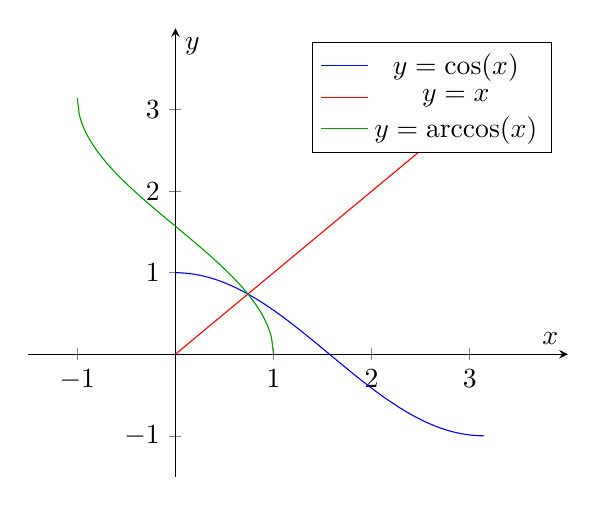
\begin{tikzpicture}
        \begin{axis}[
            axis lines = center,
            xmin=-1.5, xmax=4,
            ymin=-1.5, ymax=4,
            xlabel = $x$,
            ylabel = $y$,
            xtick={-1,0,1,2,3},
            ytick={-1,0,1,2,3},
            trig format plots=rad,
            legend pos=north east,
        ]
        % Grafico di y = cos(x) per x in [0, π]
        \addplot[
            domain=0:pi,
            samples=100,
            color=blue,
        ]
        {cos(x)};
        \addlegendentry{$y = \cos(x)$}
        
        % Grafico della retta y = x
        \addplot[
            domain=0:pi,
            samples=100,
            color=red,
        ]
        {x};
        \addlegendentry{$y = x$}
        
        % Grafico di y = arccos(x) per x in [-1, 1]
        \addplot[
            domain=-1:1,
            samples=100,
            color=darkgreen,
        ]
        {acos(x)};
        \addlegendentry{$y = \arccos(x)$}
        
        \end{axis}
    \end{tikzpicture}
\end{center}

\subsubsection{Arcsine}
The domain of the arcsine is $\forall x \in \left[-1,1\right]$ and
the range is $\dm \forall x \in \left[-\frac{\pi}{2}, \frac{\pi}{2}\right]$

\begin{center}
    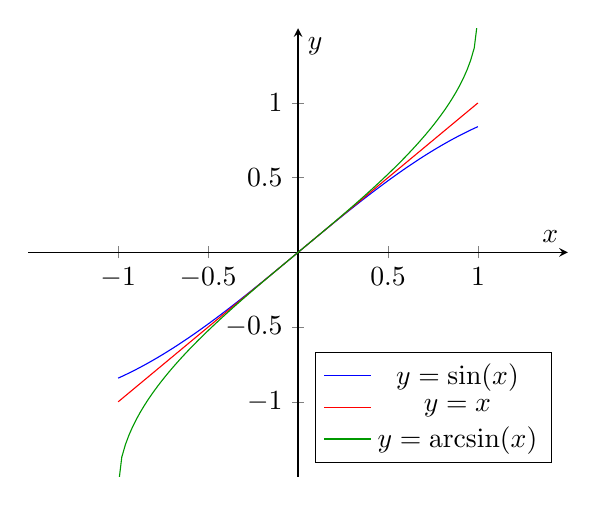
\begin{tikzpicture}
        \begin{axis}[
            axis lines = center,
            xmin=-1.5, xmax=1.5,
            ymin=-1.5, ymax=1.5,
            xlabel = $x$,
            ylabel = $y$,
            xtick={-1, -0.5, 0, 0.5, 1},
            ytick={-1, -0.5, 0, 0.5, 1},
            trig format plots=rad,
            legend pos=south east,
        ]
        % Grafico di y = \sin(x) per x in [-1, 1]
        \addplot[
            domain=-1:1,
            samples=100,
            color=blue,
        ]
        {sin(x)};
        \addlegendentry{$y = \sin(x)$}
        
        % Grafico della retta y = x
        \addplot[
            domain=-1:1,
            samples=100,
            color=red,
        ]
        {x};
        \addlegendentry{$y = x$}
        
        % Grafico di y = \arcsin(x) per x in [-1, 1]
        \addplot[
            domain=-1:1,
            samples=100,
            color=darkgreen,
        ]
        {asin(x)};
        \addlegendentry{$y = \arcsin(x)$}
        
        \end{axis}
    \end{tikzpicture}
\end{center}

\subsubsection{Arctan}
The domain is $\forall x \in \mathbb{R}$ and the range is
$\dm \forall x \in \left[-\frac{\pi}{2}, \frac{\pi}{2}\right]$

\begin{center}
    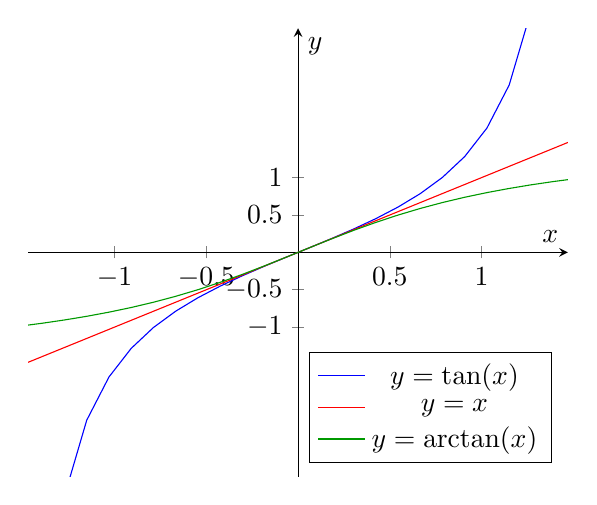
\begin{tikzpicture}
        \begin{axis}[
            axis lines = center,
            xmin=-pi/2+0.1, xmax=pi/2-0.1,
            ymin=-3, ymax=3,
            xlabel = $x$,
            ylabel = $y$,
            xtick={-1, -0.5, 0, 0.5, 1},
            ytick={-1, -0.5, 0, 0.5, 1},
            trig format plots=rad,
            legend pos=south east,
        ]
        \addplot[
            domain=-6:6,
            samples=100,
            color=blue,
        ]
        {tan(x)};
        \addlegendentry{$y = \tan(x)$}
        
        \addplot[
            domain=-6:6,
            samples=100,
            color=red,
        ]
        {x};
        \addlegendentry{$y = x$}
        
        \addplot[
            domain=-6:6,
            samples=100,
            color=darkgreen,
        ]
        {atan(x)};
        \addlegendentry{$y = \arctan(x)$}
        
        \end{axis}
    \end{tikzpicture}
\end{center}

\newpage
\subsection{Harmonic oscillation}
Let $A,B > 0$, then the function is oscillating harmonically with $t$ around $D$:

\figbox{$y = D + A\cdot \sin(Bt + \varphi)$}

\begin{center}
    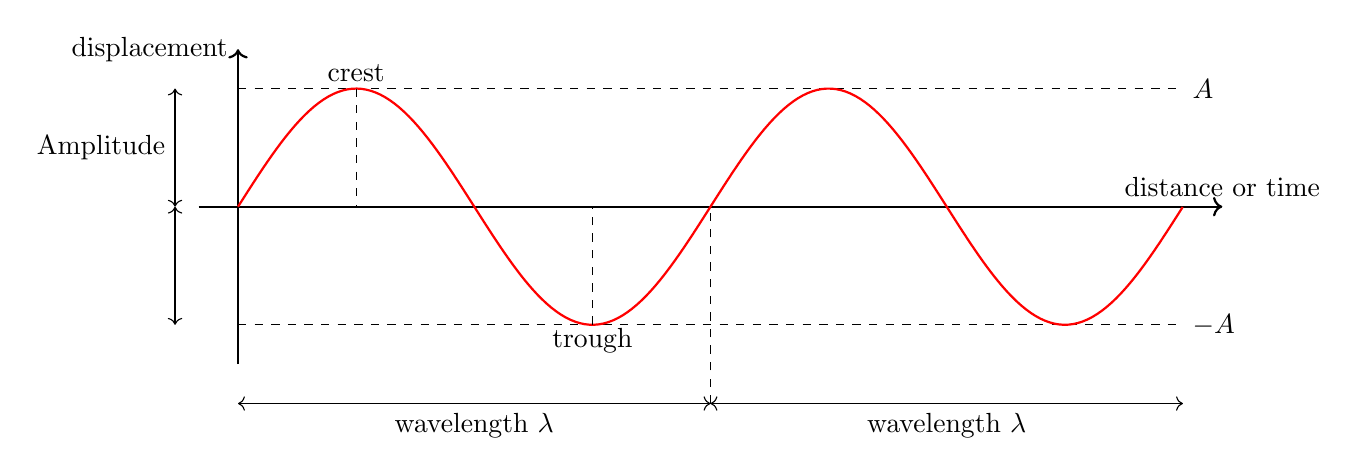
\begin{tikzpicture}[scale=1]

        \def\amplitude{1.5}
        \def\wavelength{6}
        \def\periods{2}
        \def\totalwidth{\textwidth}
        \def\scalefactor{\totalwidth / (\periods * \wavelength)}
    
        \draw[thick, ->] (-0.5, 0) -- (\periods*\wavelength + 0.5, 0) node[anchor=south] {distance or time};
        \draw[thick, ->] (0, -\amplitude-0.5) -- (0, \amplitude+0.5) node[anchor=east] {displacement};
        
        \draw[dashed] (0, \amplitude) -- (\periods*\wavelength, \amplitude) node[anchor=west] {$A$};
        \draw[dashed] (0, -\amplitude) -- (\periods*\wavelength, -\amplitude) node[anchor=west] {$-A$};
        
        \draw[thick, red, domain=0:\periods*\wavelength, samples=200, variable=\x] plot (\x, {\amplitude*sin(360*\x/\wavelength)});
                
        \draw[<->] (-.8, 0) -- (-.8, \amplitude) node[midway,left] {Amplitude};
        \draw[<->] (-.8, -\amplitude) -- (-.8, 0);
        
        \draw[dashed] (\wavelength/4, \amplitude) -- (\wavelength/4, 0);
        \node at (\wavelength/4, \amplitude + 0.2) {crest};
        \draw[dashed] (\wavelength*3/4, -\amplitude) -- (\wavelength*3/4, 0);
        \node at (\wavelength*3/4, -\amplitude - 0.2) {trough};
        
        \draw[<->] (0, -\amplitude-1) -- (\wavelength, -\amplitude-1) 
            node[midway, below] {wavelength $\lambda$};
        \draw[dashed] (\wavelength, -\amplitude-1) -- (\wavelength, 0);
    
        \draw[<->] (\wavelength, -\amplitude-1) -- (2*\wavelength, -\amplitude-1) 
            node[midway, below] {wavelength $\lambda$};
    
    \end{tikzpicture}
\end{center}

\newpage
\part{Limits}
\section{Concept of limit of a real function}
\subsection{Definition}
Let $f:\mathcal{D} \to \mathbb{R}$ be a function and $c$ a point, the limit
$\dm L=\lim_{x\to c}f(x)$ with $x$ tending to $c$ exists only if in a given
$\epsilon >0$ arbitrarily small, exists another $\delta >0$ such that:


\figbox{$0<|x-c|<\delta \implies |f(x)-L|<\epsilon$}

\subsection{Graphic interpretation}
\vspace*{.3cm}
\begin{center}
    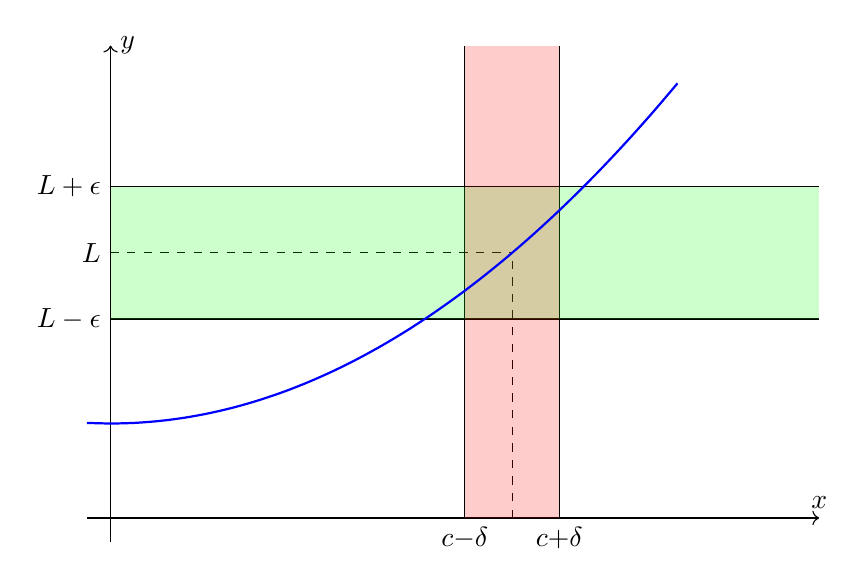
\begin{tikzpicture}[
        scale=1.2,
        declare function={
            func(\x) = \x*\x / 10 + 1;
            LimX=4.25;
            Epsilon=0.7;
            Delta=0.5;
            LimY={func(LimX)};
            Width=7.5;
            Height=5;
        }
    ]
        \draw[->] (0, -0.25) -- (0, Height) node[right] {\(y\)};
        \draw[->] (-0.25, 0) -- (Width, 0) node[above] {\(x\)};
    
        \draw[-, dashed] (LimX, 0) -- (LimX, LimY);
        \draw[-, dashed] (0, LimY) node[left] {\(L\)} -- (LimX, LimY);
    
        \draw[-] (0, {LimY + Epsilon}) node[left] {\(L + \epsilon\)} -- (Width, {LimY + Epsilon});
        \draw[-] (0, {LimY - Epsilon}) node[left] {\(L - \epsilon\)} -- (Width, {LimY - Epsilon});
    
        \draw[-] ({LimX - Delta}, 0) node[below] {\Large \(\scriptstyle c - \delta\)} -- ({LimX - Delta}, Height);
        \draw[-] ({LimX + Delta}, 0) node[below] {\Large \(\scriptstyle c + \delta\)} -- ({LimX + Delta}, Height);
    
        \fill [green, opacity=0.2] (0,{LimY - Epsilon}) rectangle (Width, {LimY + Epsilon});
        \fill [red, opacity=0.2] ({LimX - Delta}, 0) rectangle ({LimX + Delta}, Height);
    
        \draw[domain=-0.25:6, smooth, variable=\x, blue, thick] plot ({\x}, {func(\x)});
    \end{tikzpicture}
\end{center}

\section{Limit value at a finite point}
The notion of the ``limit of $f(x)$ as $x$ approaches a (finite) point
$a \in \mathbb{R}$'' is only meaningful if the point $a$ can be
approximated by points from the domain of definition of $f$. We can
precisely formulate this concept with the notion of an ``accumulation point''.

\figbox{\minipage[]{\textwidth}
\textbf{Definition} \\
Given a set $A \subset \mathbb{R}$ and a real number
$a \in \mathbb{R}$, the real number $a$ is called an
\textit{accumulation point} of the set $A$ if every open interval
of the form $(a - \delta, a + \delta)$ with $\delta > 0$ contains
infinitely many points of $A$.
\endminipage}

In the above definition, it is not required that $a$ lies in $A$.
Often, we will consider functions whose domains are unions of
intervals of the form:

\figbox{$(b, a) \cup (a, c)$}

For example, consider the function defined by $f(x) = \frac{1}{x}$, defined
on $(-\infty, 0) \cup (0, \infty)$. The point $0$ is an accumulation point of
the domain of definition of $\frac{1}{x}$.

\figbox{\minipage[]{\textwidth}
\textbf{Definition} \\
Given a real function $f$, an accumulation point $x_0$ of
$\mathcal{D}_f$, and $L \in \mathbb{R} = \mathbb{R} \cup \{\pm \infty\}$,
we say that the function $f$ has the limit $L$ as $x \to x_0$ if
$f(x)$ gets arbitrarily close to $L$, provided $x$ is sufficiently
close to (but never equal to) $x_0$.
\endminipage}

\subsection{One-sided limits}
Often, one considers limits where $x$ approaches $x_0$ from only one
direction, either from the right or from the left. In these cases,
we refer to a right-sided or left-sided limit and use the following
notations:

\figbox{$\dm \lim_{x \to x_0^+} f(x) \quad \text{or} \quad \lim_{x \to x_0, x > x_0} f(x) \quad \text{or} \quad \lim_{x \to x_0} f(x)$}

for a right-sided limit, and:

\figbox{$\dm \lim_{x \to x_0^-} f(x) \quad \text{or} \quad \lim_{x \to x_0, x < x_0} f(x) \quad \text{or} \quad \lim_{x \to x_0} f(x)$}

for a left-sided limit.

$\dm \lim_{x \to a}$ can indicate a limit as $x$ approaches an
arbitrary point (e.g., $a = x_0$ for $x_0 \in \mathbb{R}$), as well
as a one-sided limit ($a = x_0^+$ or $a = x_0^-$ for $x_0 \in \mathbb{R}$),
or a limit at infinity ($a = \pm \infty$).

\subsubsection{Graph example}
\begin{center}
    \begin{tikzpicture}[scale=1.5]
        \draw[->] (-0.5, 0) -- (3, 0) node[anchor=north] {$x$};
        \draw[->] (0, -0.5) -- (0, 2.5) node[anchor=east] {$f(x)$};
        
        \draw[domain=0:1, samples=100, thick, blue] plot (\x, {\x*\x}) node[anchor=south west] {};
        
        \draw[domain=1:2.5, samples=100, thick, blue] plot (\x, {(\x-2)*(\x-2)+1});
        
        \filldraw[blue] (1,1) circle (1pt);
        \node[anchor=south] at (1, 1.05) {1};
        
        \draw[dashed] (1, 0) -- (1, 1);
        \draw[dashed] (0, 1) -- (1, 1);
        
        \node[anchor=north east] at (0, 0) {0};
    \end{tikzpicture}
\end{center}

\section{Continuity of a function}
\figbox{\minipage[]{\textwidth-2.3cm}
\textbf{Definition} \textit{Continuity of a real function} \\
Given a real function $f : D \rightarrow C$, the function is continuous
at the point $x = c$ where $c \in D$ if:
\[
    \dm \lim_{x \to c} f(x) = f(c)
\]

and therefore, if the limit exists and is equal to the value of the
function at that point.
\endminipage}

In other words, the function is continuous at the point if the limit
exists (from both the left and right, coinciding) and the value of
the function at that point is equivalent to the value of the limit.

\begin{center}
    \begin{tikzpicture}[scale=1.5]

        \draw[->] (-3, 0) -- (3, 0) node[anchor=north] {$x$};
        \draw[->] (0, -2) -- (0, 2) node[anchor=south] {\large $f'(|x|)$} node[anchor=north east] {$y$};
    
        \draw[thick, blue] (-3, -1) -- (0, -1);
        \draw[thick, blue] (0, 1) -- (3, 1);
        
        \draw[thick, blue, fill=white] (0,1) circle (1pt);
        \draw[thick, blue, fill=white] (0,-1) circle (1pt);
        
        \node[anchor=north west] at (3, 1) {1};
        \node[anchor=south west] at (-3, -1) {-1};
        \node[anchor=north east] at (0, 0) {0};

    \end{tikzpicture}
\end{center}

\subsection{Continuity in short}
\begin{itemize}
    \item A function is said to be continuous at a point if the limit at that point exists and is equal to the value of the function at that point;
    \item A function is said to be continuous on a subinterval of the domain if it is continuous at all points in that subinterval;
    \item A function is said to be continuous if it is continuous at all points in its interval.
\end{itemize}

\newpage
\part{Derivatives}
Assume that $y=f(x)$ is a differentiable function in some interval $(a,b)$,
then we have defined the derivative function.

\section{Derivative notations}
\begin{table}[h]
    \centering
    \renewcommand{\arraystretch}{1.2}
    \begin{tabular}{|c|c|c|c>{\hspace*{-.8cm}}c|}
        \hline
        \begin{tabular}{c}
            \textbf{Type of derivative}
        \end{tabular} &
        \begin{tabular}{c}
            \textbf{First derivative}
        \end{tabular} &
        \begin{tabular}{c}
            \textbf{Second derivative}
        \end{tabular} &
        \begin{tabular}{c}
            \textbf{n-th derivative}
        \end{tabular} &
        \begin{tabular}{c}
            \phantom{} \\
            \phantom{}
        \end{tabular} \\
        \hline
        \begin{tabular}{c}
            Lagrange's notation
        \end{tabular} &
        \begin{tabular}{c}
            $f'(x)$
        \end{tabular} &
        \begin{tabular}{c}
            $f''(x)$
        \end{tabular} &
        \begin{tabular}{c}
            $f^{(n)}(x)$
        \end{tabular} &
        \begin{tabular}{c}
            \phantom{} \\
            \phantom{}
        \end{tabular} \\
        \hline
        \begin{tabular}{c}
            Leibniz's notation
        \end{tabular} &
        \begin{tabular}{c}
            $\dfrac{d}{dx} f(x)$
        \end{tabular} &
        \begin{tabular}{c}
            $\dfrac{d^2}{dx^2} f(x)$
        \end{tabular} &
        \begin{tabular}{c}
            $\dfrac{d^n}{dx^n} f(x)$
        \end{tabular} &
        \begin{tabular}{c}
            \phantom{} \\
            \phantom{}
        \end{tabular} \\
        \hline
        \begin{tabular}{c}
            Leibniz's notation\\ in a point $a$
        \end{tabular} &
        \begin{tabular}{c}
            $\dfrac{d}{dx} \left[f(x)\right]\,|\,_{x=a}$
        \end{tabular} &
        \begin{tabular}{c}
            $\dfrac{d^2}{dx^2} \left[f(x)\right]\,|\,_{x=a}$
        \end{tabular} &
        \begin{tabular}{c}
            $\dfrac{d^n}{dx^n} \left[f(x)\right]\,|\,_{x=a}$
        \end{tabular} &
        \begin{tabular}{c}
            \phantom{} \\
            \phantom{}
        \end{tabular} \\
        \hline
        \begin{tabular}{c}
            Newton's notation
        \end{tabular} &
        \begin{tabular}{c}
            $\dot{f}$
        \end{tabular} &
        \begin{tabular}{c}
            $\ddot{f}$
        \end{tabular} &
        \begin{tabular}{c}
            $\overset{\small (n)}{f}$
        \end{tabular} &
        \begin{tabular}{c}
            \phantom{} \\
            \phantom{}
        \end{tabular} \\
        \hline
    \end{tabular}
\end{table}
\vspace*{-.3cm}

\section{Definition of derivative}
The derivative of a real function $f(x)$ is defined as:

\figbox{$\dm f'(x) = \lim_{\Delta x \to 0^\pm} \frac{f(x+\Delta x)-f(x)}{\Delta x}$}

if the limit exists.

\defs{$f'(a)$, if it exists, is calld derivative of $f(x)$ at $x=a$.\\
\hspace*{1.65cm} It corresponds to the slope of the tangent line at $x=a$ to the function $y=f(x)$}

\subsection{Simplified definition (Exponentiation rule)}
Let $\forall \alpha \in \mathbb{R}$, then:
\figbox{$\dm f(x)=x^{\, \alpha} \Rightarrow f'(x)=\alpha \cdot x^{\, \alpha-1}$}

\subsection{Existence of the derivative}
The derivative exists if and only if:
\figbox{$\dm \lim_{\Delta x \to {\color{red}{0^+}}} \frac{f(x+\Delta x)-f(x)}{\Delta x} = \lim_{\Delta x \to {\color{red}{0^-}}} \frac{f(x+\Delta x)-f(x)}{\Delta x}$}

\rem{If a function is differentiable, then it is continuous:}
\figbox{Differentiable $\Longrightarrow$ Continuous}

\newpage
\section{Geometric meaning of the derivative}
\begin{minipage}{0.5\textwidth}
    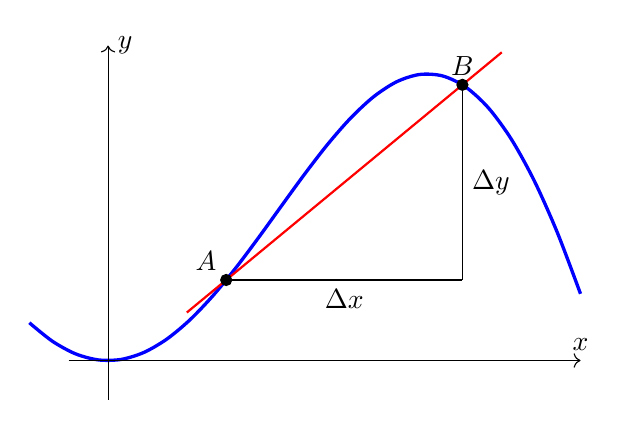
\begin{tikzpicture}[
        scale=2,
        declare function={
            func(\x) = \x*sin(\x r);
            Width=3;
            Height=2;
            Ax=0.75;
            Bx=2.25;
            SlopeMargin=0.25;
            M=(func(Bx) - func(Ax)) / (Bx - Ax);
            Q=func(Ax) - M * Ax;
            slopeFunc(\x)=\x * M + Q;
        }
    ]
        \draw[domain=-0.5:3, smooth, variable=\x, blue, very thick] plot ({\x}, {func(\x)});
        
        \draw[->] (0, -0.25) -- (0, Height) node[right] {\(y\)};
        \draw[->] (-0.25, 0) -- (Width, 0) node[above] {\(x\)};

        \draw[-] (Ax, {func(Ax)}) -- node[below] {\(\Delta x\)} (Bx, {func(Ax)});
        \draw[-] (Bx, {func(Ax)}) -- node[right] {\(\Delta y\)} (Bx, {func(Bx)});
        
        \filldraw [red, thick] ({Ax - SlopeMargin}, {slopeFunc(Ax - SlopeMargin)}) -- ({Bx + SlopeMargin}, {slopeFunc(Bx + SlopeMargin)});
        
        \filldraw (Ax,{func(Ax)}) circle (1pt) node[above left] {\(A\)};
        \filldraw (Bx,{func(Bx)}) circle (1pt) node[above] {\(B\)};
    \end{tikzpicture}
\end{minipage}
\begin{minipage}{0.5\textwidth}
    The secant of a function \(f(x)\) between a point \(A\) and \(B\) is given by:\\
    \begin{center}
        \fbox{$\dm \frac{\Delta y}{\Delta x} = \frac{f(B)-f(A)}{B-A}$}
    \end{center} \phantom{}\\

    The closer we bring \(A\) and \(B\), the smaller \(\Delta x\) becomes.
    As \(\Delta x\) decreases, the slope of the secant becomes more representative
    of the rate of change of \(f\) in the interval \([A;B]\). \\
\end{minipage}

\begin{minipage}{0.5\textwidth}
    When the \(\Delta x\) of the slope becomes infinitesimally small, we obtain the exact slope at a point (instantaneous).
    This slope is represented by the tangent line:\\

    \begin{center}
        \fbox{$\dm \lim_{\Delta x \to 0} \frac{\Delta y}{\Delta x}$}
    \end{center}

\end{minipage}
\begin{minipage}{0.5\textwidth}
    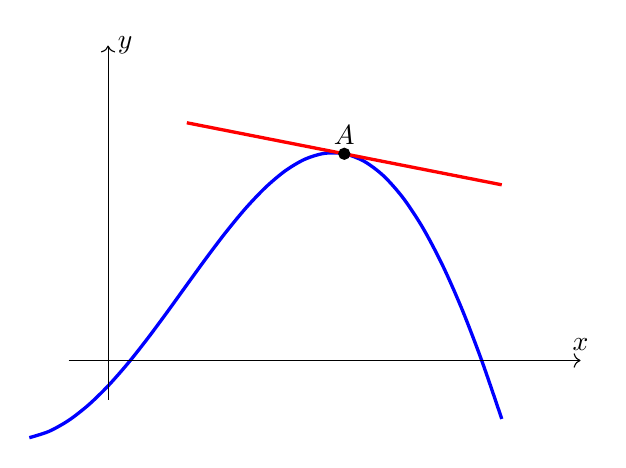
\begin{tikzpicture}[
        scale=2,
        declare function={
            func(\x) = (\x+0.6)*sin((\x+0.6) r)-0.5;
            Width=3;
            Height=2;
            Ax=1.5;
            slope = -0.19697;
        }
    ]
        \draw[domain=-0.5:2.5, smooth, variable=\x, blue, very thick] plot ({\x}, {func(\x)});
        
        \draw[->] (0, -0.25) -- (0, Height) node[right] {\(y\)};
        \draw[->] (-0.25, 0) -- (Width, 0) node[above] {\(x\)};

        \draw[domain=0.5:2.5, smooth, variable=\x, red, very thick] plot ({\x}, {slope * \x + func(Ax) - slope * Ax});
        
        \filldraw (Ax,{func(Ax)}) circle (1pt) node[above] {\(A\)};
    \end{tikzpicture}
\end{minipage}

\begin{minipage}{0.5\textwidth}
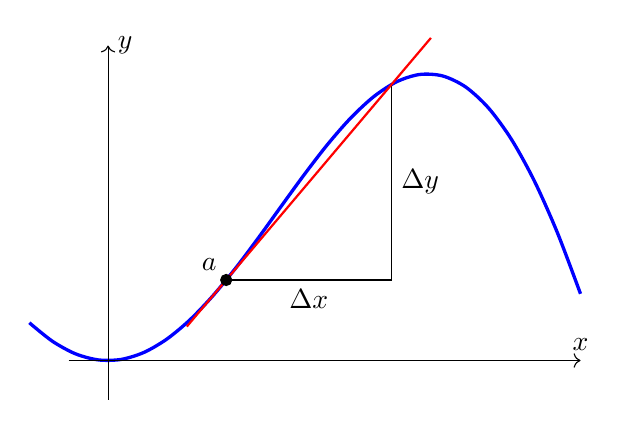
\begin{tikzpicture}[
    scale=2,
    declare function={
        func(\x) = \x*sin(\x r);
        Width=3;
        Height=2;
        Ax=0.75;
        Bx=1.8;
        SlopeMargin=0.25;
        M=(func(Bx) - func(Ax)) / (Bx - Ax);
        Q=func(Ax) - M * Ax;
        slopeFunc(\x)=\x * M + Q;
    }
]
    \draw[domain=-0.5:3, smooth, variable=\x, blue, very thick] plot ({\x}, {func(\x)});
    
    \draw[->] (0, -0.25) -- (0, Height) node[right] {\(y\)};
    \draw[->] (-0.25, 0) -- (Width, 0) node[above] {\(x\)};

    \draw[-] (Ax, {func(Ax)}) -- node[below] {\(\Delta x\)} (Bx, {func(Ax)});
    \draw[-] (Bx, {func(Ax)}) -- node[right] {\(\Delta y\)} (Bx, {func(Bx)});
    
    \filldraw [red, thick] ({Ax - SlopeMargin}, {slopeFunc(Ax - SlopeMargin)}) -- ({Bx + SlopeMargin}, {slopeFunc(Bx + SlopeMargin)});

    \filldraw (Ax,{func(Ax)}) circle (1pt) node[above left] {\(a\)};
\end{tikzpicture}
\end{minipage}
\begin{minipage}{0.5\textwidth}
The derivative of a function \(f(x)\) is therefore another function, \(f'(x)\), which
represents the rate of change of \(f(x)\) at every point. In other words, \(f'(x)\)
represents the slope of the tangent at each \(x\) of \(f(x)\).
This is precisely represented by the definition of the derivative, which is the slope
\(\frac{\Delta y}{\Delta x}\) calculated with the limit of \(\Delta x \to 0\).
\end{minipage}

\subsection{Equation of the tangent line}
When $f'(x)$ is defined, $p = \left(x, f(x)\right)$, and $p \in$ tangent line, then:
\figbox{$\dm y - f(a) = f'(a) \cdot (x-a)$}

\section{Bernoulli -- de l'Hôpital Theorem}
Bernulli -- de l'Hôpital theorem is applicable \textbf{only if} the function
results in an indeterminate form.

\subsection{The 7 indeterminate forms}

The seven indeterminate forms are:
\figbox{$\frac{0}{0}, \quad \frac{\infty}{\infty}, \quad 0 \cdot \infty, \quad
        \infty - \infty, \quad 0^0, \quad \infty^0, \quad 1^\infty$}

\newpage
\subsection{Statement of the theorem}
Let us consider two real functions $f(x)$ and $g(x)$ that are differentiable
in a neighborhood of $x_0\in\mathbb{R}$ (not necessarily at $x_0$).

If $\dm \lim_{x \to x_0} \frac{f(x_0)}{g(x_0)}$ results in an indeterminate form, then:

\figbox{$\dm \lim_{x \to x_0} \frac{f(x)}{g(x)} = \lim_{x \to x_0} \frac{f'(x)}{g'(x)}$}

if the limit exists.

\section{Derivation rules}
\subsection{Normal cases}
Let $y=f(x)$ and $y=g(x)$ be two derivable functions, then:

\subsubsection{Linearity}
Let $c \in \mathbb{R}$, then:
\figbox{$\dm \frac{d}{dx}\left[c \cdot f(x)\right] = c\cdot \frac{d}{dx}\left[f(x)\right]$}

\subsubsection{Sum and subtraction}
\figbox{$\dm f'(x) \pm g'(x) = \frac{d}{dx}\left[f(x) \pm g(x)\right]$}

\subsubsection{Multiplication}
\figbox{$\dm \frac{d}{dx}\left[f(x) \cdot g(x)\right] = f'(x)\cdot g(x) + f(x)\cdot g'(x)$}

\subsubsection{Difference}
\figbox{$\dm \frac{d}{dx}\left[\frac{f(x)}{g(x)}\right] = \frac{f'(x)\cdot g(x) - f(x)\cdot g(x)}{\left(g(x)\right)^2}$}

\subsubsection{Exponential}
Let $a > 0$, then:
\figbox{$\dm \frac{d}{dx}\left[a^x\right] = a^x\cdot \ln(a)$}

\subsubsection{Composite function (Chain rule)}
\figbox{$\dm \frac{d}{dx}\left[f(g(x))\right] = f'(g(x))\cdot g'(x)$}

\newpage
\subsubsection{Inverse function}
\figbox{$\dm \frac{d}{dx}\left[f^{-1}(x)\right] = \frac{1}{f'(f^{-1}(x))}$}

\subsubsection{Trigonometric functions}
\begin{center}
    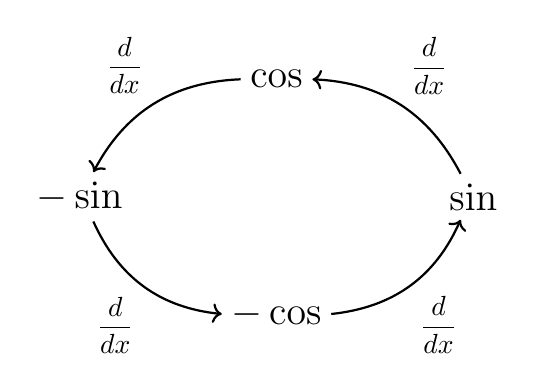
\begin{tikzpicture}[node distance=3cm, auto]
        \node (cos) at (0, 1.5) {\Large$\cos$};
        \node (sin) at (2.5, 0) {\Large$\sin$};
        \node (neg_cos) at (0, -1.5) {\Large$-\cos$};
        \node (neg_sin) at (-2.5, 0) {\Large$-\sin$};
    
        \draw[<-, thick] (cos) to[bend left] node[midway, above right] {$\dfrac{d}{dx}$} (sin);
        \draw[<-, thick] (sin) to[bend left] node[midway, below right] {$\dfrac{d}{dx}$} (neg_cos);
        \draw[<-, thick] (neg_cos) to[bend left] node[midway, below left] {$\dfrac{d}{dx}$} (neg_sin);
        \draw[<-, thick] (neg_sin) to[bend left] node[midway, above left] {$\dfrac{d}{dx}$} (cos);
    \end{tikzpicture}
    
    \fbox{\hspace*{-.7cm}
      \begin{minipage}{0.28\textwidth}\vspace*{-.35cm}
        \[
          (\sec x)' = \sec x \tan x 
        \]
        \[
          (\tan x)' = \frac{1}{\cos^2(x)}
        \]
        \[
          (\arcsin x)' = \frac{1}{\sqrt{1 - x^2}}
        \]
        \[
          (\arctan x)' = \frac{1}{1 + x^2}
        \]
      \end{minipage}%
      \begin{minipage}{0.27\textwidth}\vspace*{-.35cm}
        \[
          (\csc x)' = -\csc x \cot x
        \]
        \[
          (\cot x)' = \frac{-1}{\sin^2(x)}
        \]
        \[
          (\arccos x)' = \frac{-1}{\sqrt{1 - x^2}}
        \]
        \[
          (\text{arccot } x)' = \frac{-1}{1 + x^2}
        \]
      \end{minipage}
    }
\end{center}

\subsection{Particular cases}
\begin{enumerate}
    \item \[f(x) = g(x)^\alpha \Longrightarrow f'(x)=\alpha \cdot g'(x) \cdot g(x)^{\alpha -1}
    \\ \text{i.g.: } \left(x^2+1\right)^4 \Longrightarrow 8x \cdot \left(x^2+1\right)^3\]
    \item \[f(x) = e^{g(x)} \Longrightarrow f'(x)=g'(x)\cdot e^{g(x)}\]
    \item \[f(x) = \frac{1}{g(x)} \Longrightarrow f'(x)=\frac{-g'(x)}{\left(g(x)\right)^2}\]
\end{enumerate}

\subsection{Physical application}

\subsubsection{Average acceleration $a_{av}$}
\figbox{$\dm a_{av} := \frac{v(t_f)-v(t_i)}{t_f-t_i}$}

\subsubsection{Instant acceleration $a(t)$}
\figbox{$\dm a(t) := v'(t) = \lim_{t \to 0} \frac{v(t + h)-v(t)}{\Delta t}$}

\newpage
\section{Linearization}
\subsection{The linearization principle}
In a very small neighborhood around a point $a$, we can assume that
the function is linear at that point.

\subsection{Tangent line approximation}
In this case, assuming that the function is linear, we can use the
tangent line equation:
\figbox{$\dm f(x) = f(a)+f'(a)\cdot (x-a)$}

\subsection{Error function}
The error of the approximation is given by the difference between
the exact function and the linearization:
\figbox{$E(x) = d(f(x) \mid f_{\text{lin}}(x)) = f(x)-f(a)-f'(a)\cdot(x-a)$}

\section{Monotonicity}
\subsection{Definition of monotonicity}
A real function $f$ defined on an interval $I \subset \mathcal{D}_f$ is denoted as:
\begin{itemize}
    \item \textit{strictly monotonically increasing} on $I$, if $f(x_2) > f(x_1)$ applies for all $x_1, x_2 \in I$ with $x_2 > x_1$;
    \item \textit{monotonically increasing} on $I$, if $f(x_2) \geq f(x_1)$ applies for all $x_1, x_2 \in I$ with $x_2 > x_1$;
    \item \textit{strictly monotonically decreasing} on $I$, if $f(x_2) < f(x_1)$ applies for all $x_1, x_2 \in I$ with $x_2 > x_1$;
    \item \textit{monotonically decreasing} on $I$, if $f(x_2) \leq f(x_1)$ applies for all $x_1, x_2 \in I$ with $x_2 > x_1$.
\end{itemize}

\subsubsection{Monotonicity criterion}
Let the function $f$ be differentiable on the interval $I$:
\begin{itemize}
    \item If $f'(x) > 0$ (resp. $\geq 0$) for all $x \in I$, then $f$ is strictly monotonically increasing (resp. monotonically increasing) on $I$.
    \item If $f'(x) < 0$ (resp. $\leq 0$) for all $x \in I$, then $f$ is strictly monotonically decreasing (resp. monotonically decreasing) on $I$.
    \item If $f'(x) = 0$ for all $x \in I$, then $f$ is constant on $I$.
\end{itemize}

\subsubsection{Monotonicity table}
Let $f(x)$ be differentiable, $f'(x)<0$ if $a<x<b$,\ $a,b,c \in \mathcal{D}_f$, and $a,b,c$ are critical points, then:
\\
\begin{center}
    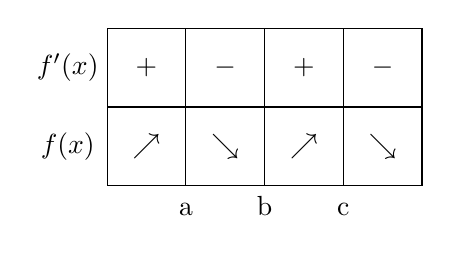
\begin{tikzpicture}
        \node at (0, 1) {$f'(x)$};
        \node at (1, 1) {$+$};
        \node at (2, 1) {$-$};
        \node at (3, 1) {$+$};
        \node at (4, 1) {$-$};
        
        \node at (0, 0) {$f(x)$};
        \node at (1, 0) {$\nearrow$};
        \node at (2, 0) {$\searrow$};
        \node at (3, 0) {$\nearrow$};
        \node at (4, 0) {$\searrow$};
        
        \draw (0.5, 1.5) -- (4.5, 1.5);
        \draw (0.5, -0.5) -- (4.5, -0.5);
        \draw (0.5, 1.5) -- (0.5, -0.5);
        \draw (4.5, 1.5) -- (4.5, -0.5);
        \draw (0.5, 0.5) -- (4.5, 0.5);

        \draw (1.5, 1.5) -- (1.5, -0.5);
        \draw (2.5, 1.5) -- (2.5, -0.5);
        \draw (3.5, 1.5) -- (3.5, -0.5);
        
        \node at (1.5, -.8) {a};
        \node at (2.5, -.75) {b};
        \node at (3.5, -.8) {c};
    \end{tikzpicture}
\end{center}

\subsection{Critical point}
Let $y_f(x)$ be a function, then we say that $x \in \mathcal{D}_f$ is
a critical point if $f'(x)=0$ or $f'(x)\uparrow$

\wrn{many critical points are local extrema, some aren't.}

\newpage
\subsection{Darboux theorem}
Let $f$ be differentiable on an interval $I$:
\begin{enumerate}
    \item find the critical points $f'(a,b)=0,\ a<b$;
    \item take a random point \textbf{between the critical points} in $c \sht a<c<b$;
    \item compute $f'(c)$.
\end{enumerate}

\figbox{
    \begin{minipage}{.36\textwidth}
        \begin{center}
            If $f'(c)>0$, then $f'(x) > 0,\ \forall x \in \left(a,b\right)$
            
            \vspace*{.1cm}
            If $f'(c)<0$, then $f'(x) < 0,\ \forall x \in \left(a,b\right)$
        \end{center}
    \end{minipage}
}

\section{Minimum and maximum}
Let a real function $f$ and a point $x_0 \in \mathcal{D}_f$ be given.

\begin{center}
    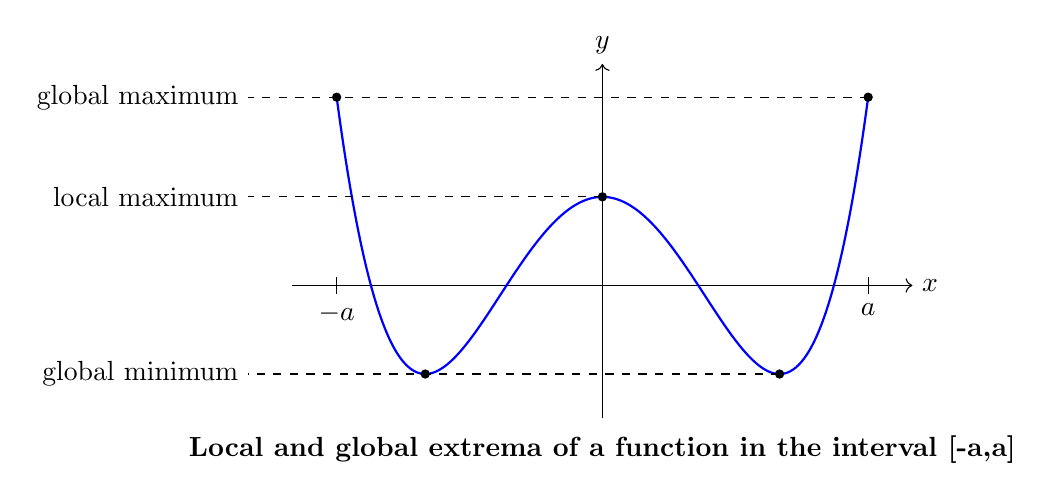
\begin{tikzpicture}[scale=1.125]
        \draw[->] (-3.5, 0) -- (3.5, 0) node[right] {$x$};
        \draw[->] (0, -1.5) -- (0, 2.5) node[above] {$y$};
    
        \draw[thick, blue, domain=-3:3, smooth, samples=200] plot (\x, {2*(0.5*\x - 1)*(0.5*\x - 1)*(0.5*\x + 1)*(0.5*\x + 1) - 1});
    
        \fill (0, 1) circle (1.5pt) node[below right] {};
        \draw[dashed] (0, 1) -- (-4, 1) node[left] {local maximum};
    
        \fill (-2, -1) circle (1.5pt) node[below left] {};
        \fill (2, -1) circle (1.5pt) node[below right] {};
        \draw[dashed] (2, -1) -- (-4, -1) node[left] {global minimum};

        \fill (3, 2.125) circle (1.5pt) node[right] {};
        \fill (-3, 2.125) circle (1.5pt) node[right] {};
        \draw[dashed] (3, 2.125) -- (-4, 2.125) node[left] {global maximum};
    
        \draw (-3, 0.1) -- (-3, -0.1) node[below] {$-a$};
        \draw (3, 0.1) -- (3, -0.1) node[below] {$a$};
        
        \node at (0,-1.85) {\textbf{Local and global extrema of a function in the interval [-a,a]}};
    \end{tikzpicture}
\end{center}

\subsection{Local extrema}
\subsubsection{Local maximum}
The function $f$ has a \textbf{local maximum point} at point $x_0$ if
there is an open neighborhood $U(x_o)$ such that:
\figbox{$f(x) \leq f(x_0),\ \forall x \in U(x_0) \cap \mathcal{D}_f$}

\subsubsection{Local minimum}
The function $f$ has a \textbf{local minimum point} at point $x_0$ if
there is an open neighborhood $U(x_o)$ such that:
\figbox{$f(x) \geq f(x_0),\ \forall x \in U(x_0) \cap \mathcal{D}_f$}

\subsection{Global extrema}
\subsubsection{Global maximum}
The function $f$ has a \textbf{global maximum} at point $x_0$ if:
\figbox{$f(x) \leq f(x_0),\ \forall x \in \mathcal{D}_f$}

\subsubsection{Global minimum}
The function $f$ has a \textbf{global minimum} at point $x_0$ if:
\figbox{$f(x) \geq f(x_0),\ \forall x \in \mathcal{D}_f$}

\subsection{Extrema tricks}
\begin{itemize}
    \item If $f'(x_0) = 0$ and $f''(x_0) < 0$ are valid, $f$ has a local maximum in $x_0$;
    \item If $f'(x_0) = 0$ and $f''(x_0) > 0$ are valid, $f$ has a local minimum in $x_0$.
\end{itemize}

\wrn{This method does not work because if $f''(x_0) = 0$, then we may have either a local maximum,\\ \hspace*{1.45cm} minimum or a stationary point.}

\section{Higher derivatives}
We define $y=f^{(n)}(x)$ as the derivative of $y=f^{(n-1)}(x)$.

\rem{Derivatives will be written with the Lagrange's notation and roman numbers, i.g.: $f''''(x) \to f^{\rom{4}}(x)$}

\subsection{Concavity}
\subsubsection{Definition of Concavity}
The concavity of a function $f(x)$ describes the direction of its curvature, which can be
upward when $f''(x) > 0$ or downward when $f''(x) < 0$.

Additionally, the concavity can be increasing when near the concavity $f'(x) > 0$ and 
decreasing when $f'(x) < 0$.

\begin{minipage}{0.5\textwidth}
    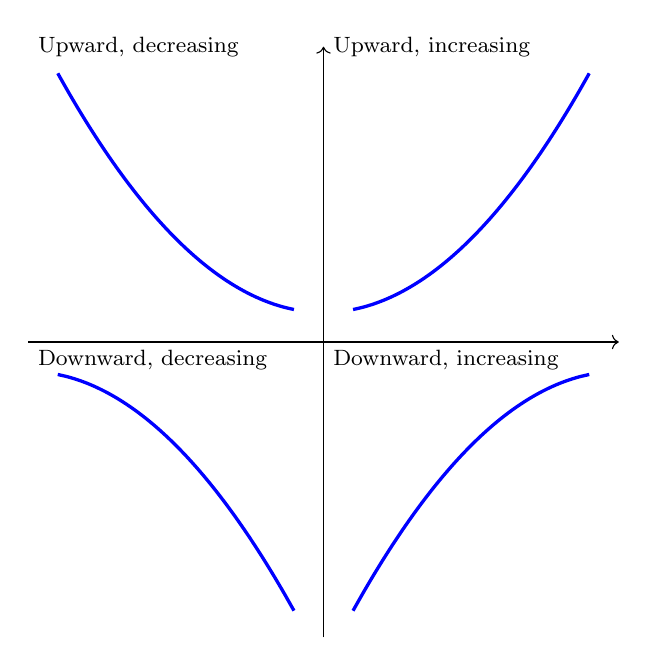
\begin{tikzpicture}[
        scale=1.5,
        declare function={
            func(\x) = \x*\x*0.4;
            Width=5;
            Height=5;
        }
    ]

        \draw[domain=0.25:2.25, smooth, variable=\x, blue, very thick] plot ({\x}, {func(\x - 2.5) + 2.75});
        \draw[domain=2.75:4.75, smooth, variable=\x, blue, very thick] plot ({\x}, {func(\x - 2.5) + 2.75});
        \draw[domain=0.25:2.25, smooth, variable=\x, blue, very thick] plot ({\x}, {-func(\x) + 2.25});
        \draw[domain=2.75:4.75, smooth, variable=\x, blue, very thick] plot ({\x}, {-func(\x - 5) + 2.25});
        
        \node[right] at (0, Height) {\footnotesize Upward, decreasing};
        \node[right] at ({Width / 2}, Height) {\footnotesize Upward, increasing};
        \node[right] at (0, Height / 2 - 0.15) {\footnotesize Downward, decreasing};
        \node[right] at ({Width / 2}, {Height / 2 - 0.15}) {\footnotesize Downward, increasing};
        
        \draw[->] ({Width / 2}, 0) -- ({Width / 2}, Height);
        \draw[->] (0, {Height / 2}) -- (Width, {Height  / 2});
    \end{tikzpicture}
\end{minipage}
\begin{minipage}{0.5\textwidth}
    \phantom{ } \\
    \begin{itemize}
        \item $f(x)$ is \textbf{concave upward} in an interval $I$ if all the tangents in $I$ are below the graph.
        \item $f(x)$ is \textbf{concave downward} in an interval $I$ if all the tangents in $I$ are above the graph.
    \end{itemize}
    \hphantom{ } \\
    \begin{itemize}
        \item If $f''(x) > 0$ for all $x$ in an interval $I$, then $f(x)$ is concave upward in $I$.
        \item If $f''(x) < 0$ for all $x$ in an interval $I$, then $f(x)$ is concave downward in $I$.
    \end{itemize}
\end{minipage}

\subsection{Inflection point}
An inflection point for $y=f(x)$ is a point $x_0 \in \mathcal{D}_f$ where the function is continuous and its concavity changes.

For any inflection point, $f''(x) = 0$.

\begin{figure}[ht!]
    \centering
    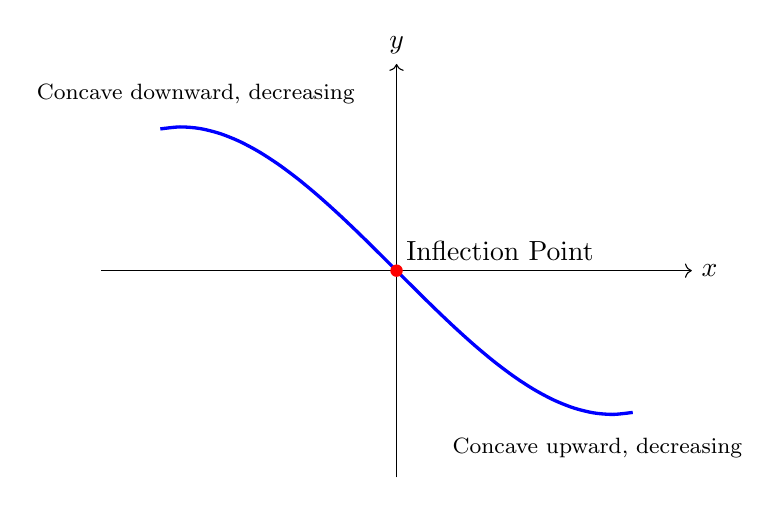
\begin{tikzpicture}[
        scale=1.5,
        declare function={
            func(\x) = 0.1 * (\x)^3 - \x;
            Width=5;
            Height=5;
        }
    ]
        
        \draw[->] (-2.5, 0) -- (2.5, 0) node[right] {$x$};
        \draw[->] (0, -1.75) -- (0, 1.75) node[above] {$y$};

        \draw[domain=-2:2, smooth, variable=\x, blue, very thick] plot ({\x}, {func(\x)});

        \fill[red] (0, {func(0)}) circle (1.5pt);
        \node[above right] at (0, {func(0)}) {Inflection Point};

        \node at (-1.7, 1.5) {\footnotesize Concave downward, decreasing};
        \node at (1.7, -1.5) {\footnotesize Concave upward, decreasing};
    \end{tikzpicture}
\end{figure}

\wrn{$f''(x_0) = 0 \not\Rightarrow x_0$ is an inflection point.}

\subsection{Curvature of a function}
Let $y=f(x)$ be a derivable function in a point $x_0$, then:
\figbox{$\dm \kappa = \frac{f''(x_0)}{(1+(f'(x_0))^2)^{3/2}}$}

\subsubsection{Radius of curvature}
The radius of curvature is given by the following formula:
\figbox{$\dm r_p = \frac{1}{\left|\kappa\right|}$}

\subsubsection{Graphical example}
\begin{figure}[ht!]
    \centering
    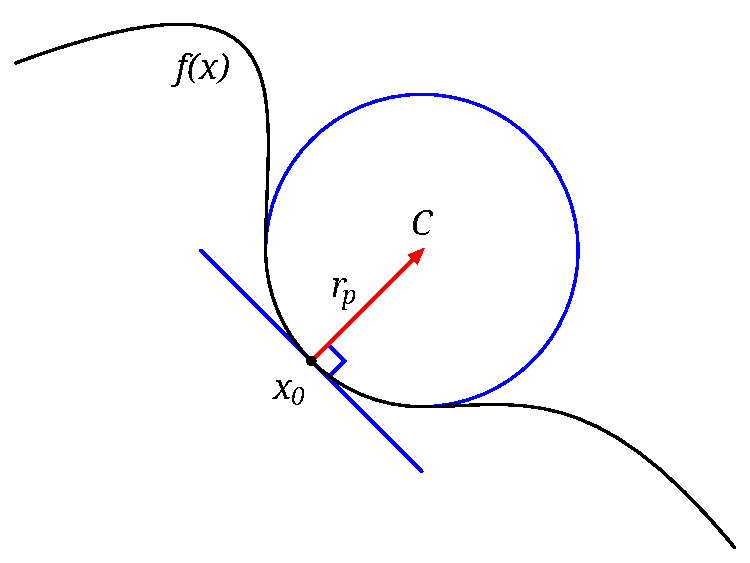
\includegraphics[width=.5\textwidth]{media/Osculating.pdf}
\end{figure}

\begin{itemize}
    \item $C =$ Center of the circle
    \item $r_p =$ Radius of curvature
    \item $x_0 =$ Specific point
\end{itemize}

\newpage
\part{Integrals}
\section{Definite integral}
Let $f(x)$ be a continuous function defined on an interval $[a, b]$.  
The definite integral from $a$ to $b$ represents the net area under the curve of $f(x)$  
between $x = a$ and $x = b$, considering areas above the x-axis as positive  
and those below as negative.
\begin{center}
    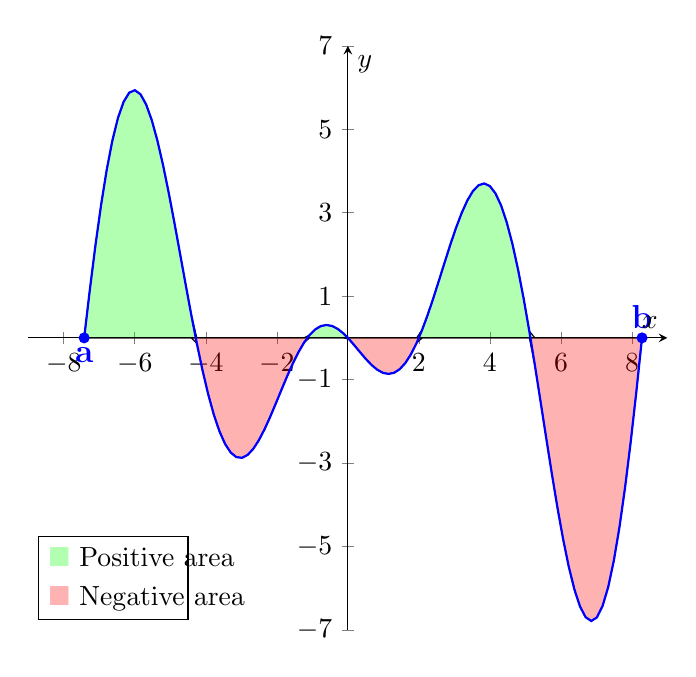
\begin{tikzpicture}
        \begin{axis}[
            domain=-7.42478:8.28319,
            samples=100,
            axis x line=middle,
            axis y line=middle,
            xlabel={$x$},
            ylabel={$y$},
            xtick={-10,-8,...,10},
            ytick={-7,-5,...,7},
            ymin=-7, ymax=7,
            xmin=-9, xmax=9,
            width=.8\textwidth,
            height=9cm,
            legend pos=north west
            ]
            \addplot [
            domain=-7.42478:8.28319,
            samples=100,
            fill=green,
            fill opacity=0.3
            ]
            {max(0, sin(deg(x-2))*x)} \closedcycle;

            \addplot [
            domain=-7.42478:8.28319,
            samples=100,
            fill=red,
            fill opacity=0.3
            ]
            {min(0, sin(deg(x-2))*x)} \closedcycle;

            \addplot [
            domain=-7.42478:8.28319,
            samples=100,
            thick,
            color=blue
            ]
            {sin(deg(x-2))*x};

            \node[right] at (-8.7,-5.25) {{\color{green!30}{$\blacksquare$}} Positive area};
            \node[right] at (-8.7,-6.25) {{\color{red!30}{$\blacksquare$}} Negative area};
            \draw (-8.7,-4.75) rectangle (-4.5,-6.75);


            \fill[blue] (-7.42478, 0) circle (2pt) node[below,blue] {\large \textbf{a}};
            \fill[blue] (8.28319, 0) circle (2pt) node[above,blue] {\large \textbf{b}};
        \end{axis}
    \end{tikzpicture}
\end{center}

\subsection{Definite integral cases}
Let $f(x)$ be a continuous function in $\mathbb{R} \to \mathbb{R}$, then
we have three possible cases:

\subsubsection{First case}
When $a<b$:
\figbox{$\integral[a][b][f(x)][x] = F(x)\Big|^b_a + C$}

\subsubsection{Second case}
When $a>b$:
\figbox{$\integral[a][b][f(x)][x] = -\integral[b][a][f(x)][x]$}

\subsubsection{Third case}
When $a=b,\ \forall a \in \mathbb{R}$:
\figbox{$\integral[a][a][f(x)][x]=0$}

\subsection{How to calculate definite integrals}
\begin{wrapfigure}{l}{7.5cm}
    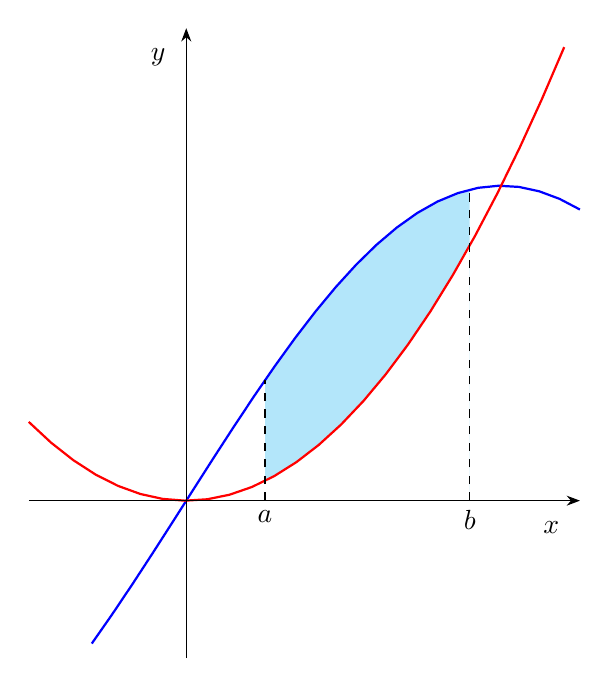
\begin{tikzpicture}[x=4cm, y=4cm, >=Stealth, declare function={
        func1(\x) = sin(3.14*\x/2 r);
        func2(\x) = \x*\x;
        a=0.25;
        b=0.9;
    }]
        % area under func1 
        \fill[cyan!30!white] plot[domain=a:b] (\x,{func1(\x)}) -- plot[domain=b:a] (\x,{0}) -- cycle;
        
        % area under func2
        \fill[white] plot[domain=a:b] (\x,{func2(\x)}) -- plot[domain=b:a] (\x,{0}) -- cycle;
        
        % func1
        \draw[blue, -, thick] plot[domain=-0.3:1.25] (\x,{func1(\x)});
        
        % func2
        \draw[red, -, thick]  plot[domain=-0.5:1.2] (\x,{func2(\x)});

        \draw[-, dashed] (a, 0) node[below] {\(a\)} -- (a, {func1(a)});
        \draw[-, dashed] (b, 0) node[below] {\(b\)} -- (b, {func1(b)});

        \draw[->] (-.5,0) -- (1.25, 0)
            node[below left=4pt] {\(x\)};
        \draw[->] (0,-.5) -- (0,1.5)
            node[below left=4pt] {\(y\)};
    \end{tikzpicture}
\end{wrapfigure}

\phantom{}

Given a function \(y=f(x)\) and \(y=g(x)\), the area enclosed by the two functions
in the interval \(I=[a;b]\) is given by:

\begin{center}
    \fbox{$\dm A=\integral[a][b][f(x)-g(x)][x]$}
\end{center} \phantom{}\\
assuming that \(f(x)\geq g(x)\) when \(x\in I\).

\vspace*{.1cm}
If \(f(x)<g(x)\) for some \(x\in I\), this formula will not work.

However, it is still possible to split the integral into multiple integrals at each point where \(f(x) - g(x)\) changes sign.
To remove the sign constraint, we could say:

\begin{center}
    \fbox{$\dm A = \integral[a][b][|f(x)-g(x)|][x]$}
\end{center} \phantom{}\\
\wrapfill

\vspace*{-4.5cm}
\subsection{Riemann sum}
Let $f: [a,b] \to \mathbb{R}$, :
\figbox{$\dm R_n := \sum_{i=0}^{n-1} f(x_i) \cdot \Delta x$}

with:
\begin{itemize}
    \item $\Delta x = \dfrac{b-a}{n},\ n \in \mathbb{N}$
    \item $x_i = a + i \cdot \Delta x$
\end{itemize}

\wrn{there are functions that are not integrable in the Riemann sense, such as sgn$(x)$}

\subsubsection{Statement of the theorem}
\figbox{$\integral[a][b][f(x)][x] = \lim_{n \to +\infty} R_n$}

\subsubsection{Sigma notaiton}
\figbox{$\dm R_n = \sum_{i=0}^{n-1} \frac{1}{n} f(x_i) = \sum_{i=0}^{n-1} \frac{1}{n} f\left(1 + \frac{i}{n}\right) = \sum_{i=0}^{n-1} \frac{1}{n} \left(1 + \frac{i}{n}\right)^2$}

\newpage
\subsubsection{Graphic interpretation}
The definite integral can be considered as the Riemann integral, which can be defined
with the infinitesimal sum of rectangles with a base tending to 0 and a height equal to a point
within the base:
\begin{center}
    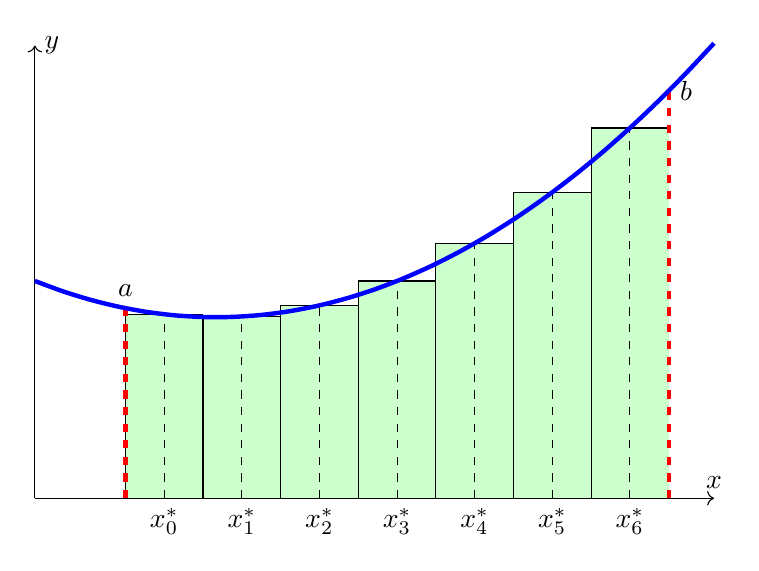
\begin{tikzpicture}[
        scale=1.15,
        declare function={
            func(\x) = 0.1 * (\x - 2) * (\x - 2) + 2;
            Width=7.5;
            Height=5;
            A = 1;
            B = 7;
            N = 7;
            Delta = {(B-A) / N};
        }
    ]
        \draw[->] (0, 0) -- (0, Height) node[right] {\(y\)};
        \draw[->] (0, 0) -- (Width, 0) node[above] {\(x\)};

        \pgfmathtruncatemacro\END{N-1}
        \foreach \x in {0,1,...,\END} {
            % rectangle
            \fill [green, opacity=0.2]
                ({A + Delta * \x}, 0) rectangle ({A + Delta * (\x+1)}, {func(A + Delta * (\x + 0.5))});
            
            \draw[-] ({A + Delta * \x}, 0)
                -- ({A + Delta * \x}, {func(A + Delta * (\x + 0.5))});

            \draw[-, dashed] ({A + Delta * (\x + 0.5)}, 0)
                node[below] {\(x_{\x}^*\)}
                -- ({A + Delta * (\x + 0.5)}, {func(A + Delta * (\x + 0.5))});

            % line over rectangle
            \draw[-] ({A + Delta * \x}, {func(A + Delta * (\x + 0.5))})
                -- ({A + Delta * (\x+1)}, {func(A + Delta * (\x + 0.5))});
        }

        \draw[-, dashed, red, ultra thick] (A, 0) -- (A, {func(A)}) node[above, black] {\(a\)};
        \draw[-, dashed, red, ultra thick] (B, 0) -- (B, {func(B)}) node[right, black] {\(b\)};

        \draw[domain=0:Width, smooth, variable=\x, blue, ultra thick] plot ({\x}, {func(\x)});
    \end{tikzpicture}
\end{center}

\subsection{Integration rules}
\subsubsection{Linearity}
Let $\lambda \in \mathbb{R}$, then:
\figbox{$\integral[][][\lambda f(x)][x] = \lambda \integral[][][f(x)][x]$} 

\subsubsection{Sum and subtraction}
\figbox{$\integral[][][[f(x) \pm g(x)]][x] = \integral[][][f(x)][x] \pm \integral[][][g(x)][x]$}

\subsection{Integral with infinite bounds}
\subsubsection{When upper bound is $+\infty$}
\figbox{$\integral[a][\infty][f(x)][x] = \lim_{t \to \infty} \integral[a][t][f(x)][x]$}

\subsubsection{When lower bound is $-\infty$}
\figbox{$\integral[-\infty][b][f(x)][x] = \lim_{t \to -\infty} \integral[t][b][f(x)][x]$}

\subsubsection{When bounds are $\infty$}
\figbox{$\integral[-\infty][\infty][f(x)][x] = \lim_{t \to -\infty} \integral[t][a][f(x)][x] + \lim_{t \to \infty} \integral[a][t][f(x)][x]$}

\newpage
\section{Indefinite integral}
We denote the \textbf{set} of all antiderivatives of a function $f$ as
an \textit{indefinite integral} of $f$. This is written as:
\begin{center}
    $\integral[][][f(x)][x]$
\end{center}

with no integration limits specified.

\subsection{Fundamental theorem of calculus}
Let $F:[a,b] \to \mathbb{R}$ a continuous function, differentiable in $(a,b)$.\\
Let $f(x)=F'(x)$ and $\forall C \in \mathbb{R}$, then:
\figbox{$\integral[a][b][f'(x)][x] = f(b) - f(a)$}

\rem{Since $F'(x) = f(x)$, we have infinite possible primitives, which are distinguished by the constant $C$.}

\subsection{Second fundamental theorem of differential and integral calculus}
If $f:[a,b] \to \mathbb{R}$ is continuous and $x_0 \in [a,b]$,
then $\forall x \in [a,b]$:
\figbox{$F_0 (x) = \integral[x][x_0][f(t)][t]$}










\end{document}
